\chapter{Security of IP Networks}
\cite{04_NetSec}

\section{Network Access Control}

\begin{multicols}{2}
    \raggedright
    \begin{center}
        \textbf{Past Method}
    \end{center}
    In the past, connections were established via dial-up lines, where a computer used a modem to dial a phone number to an Internet Service Provider (ISP). The ISP would then contact the Network Access Server (NAS) and, if feasible, connect the computer to the Internet.
    \begin{figure}[H]
        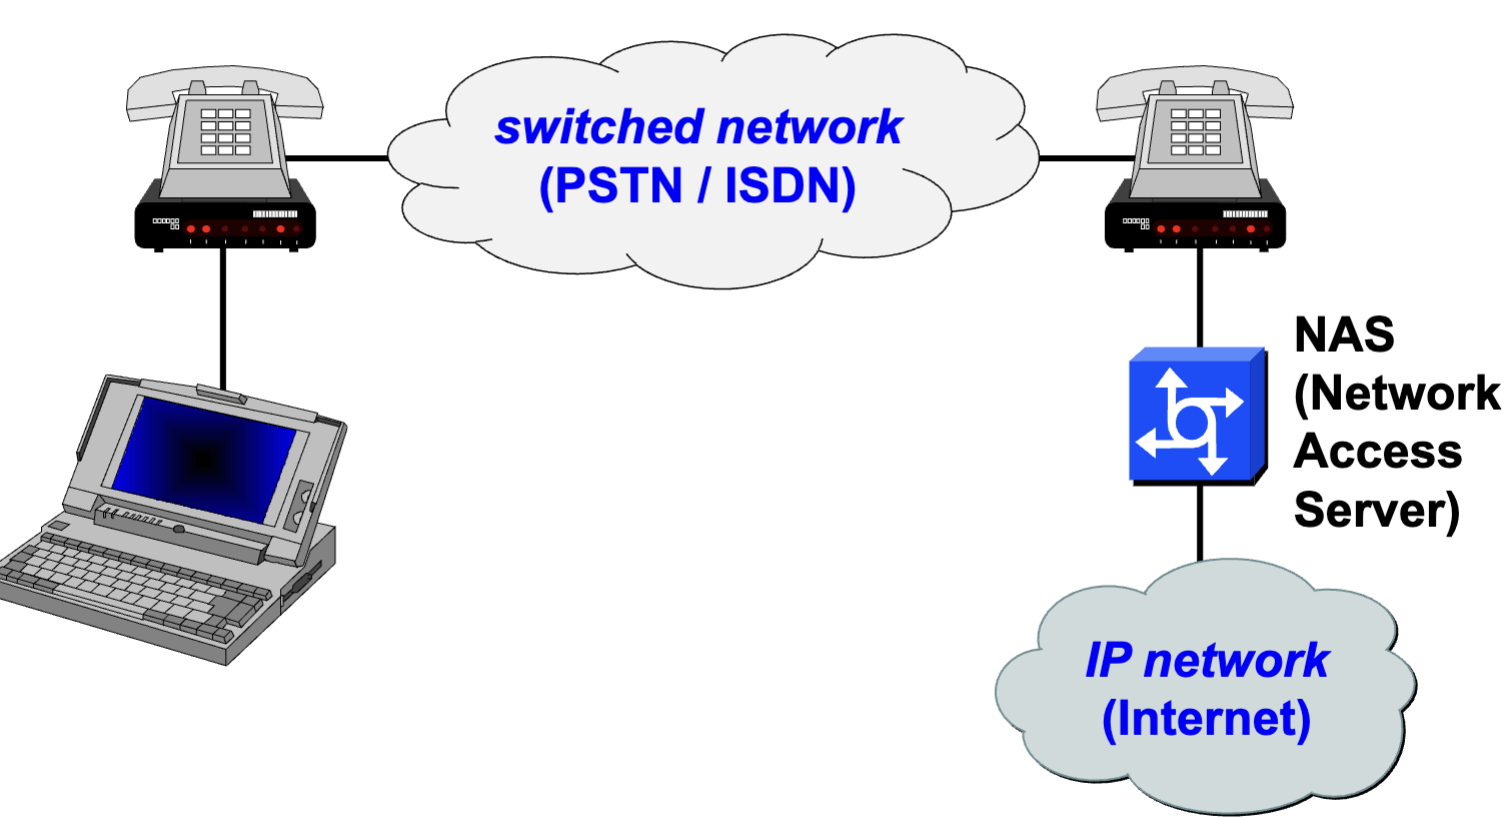
\includegraphics[width=\linewidth]{Images/NetSec/NetAccessOld.png}
        \caption{Network access, past method}
    \end{figure}
    \columnbreak
    \begin{center}
        \textbf{Modern Method}
    \end{center}
    Nowadays, many devices can connect to the Core Network through various types of connections, including fiber optics, cellular networks, and Wi-Fi. The core network serves as the backbone for modern communication networks.
    \begin{figure}[H]
        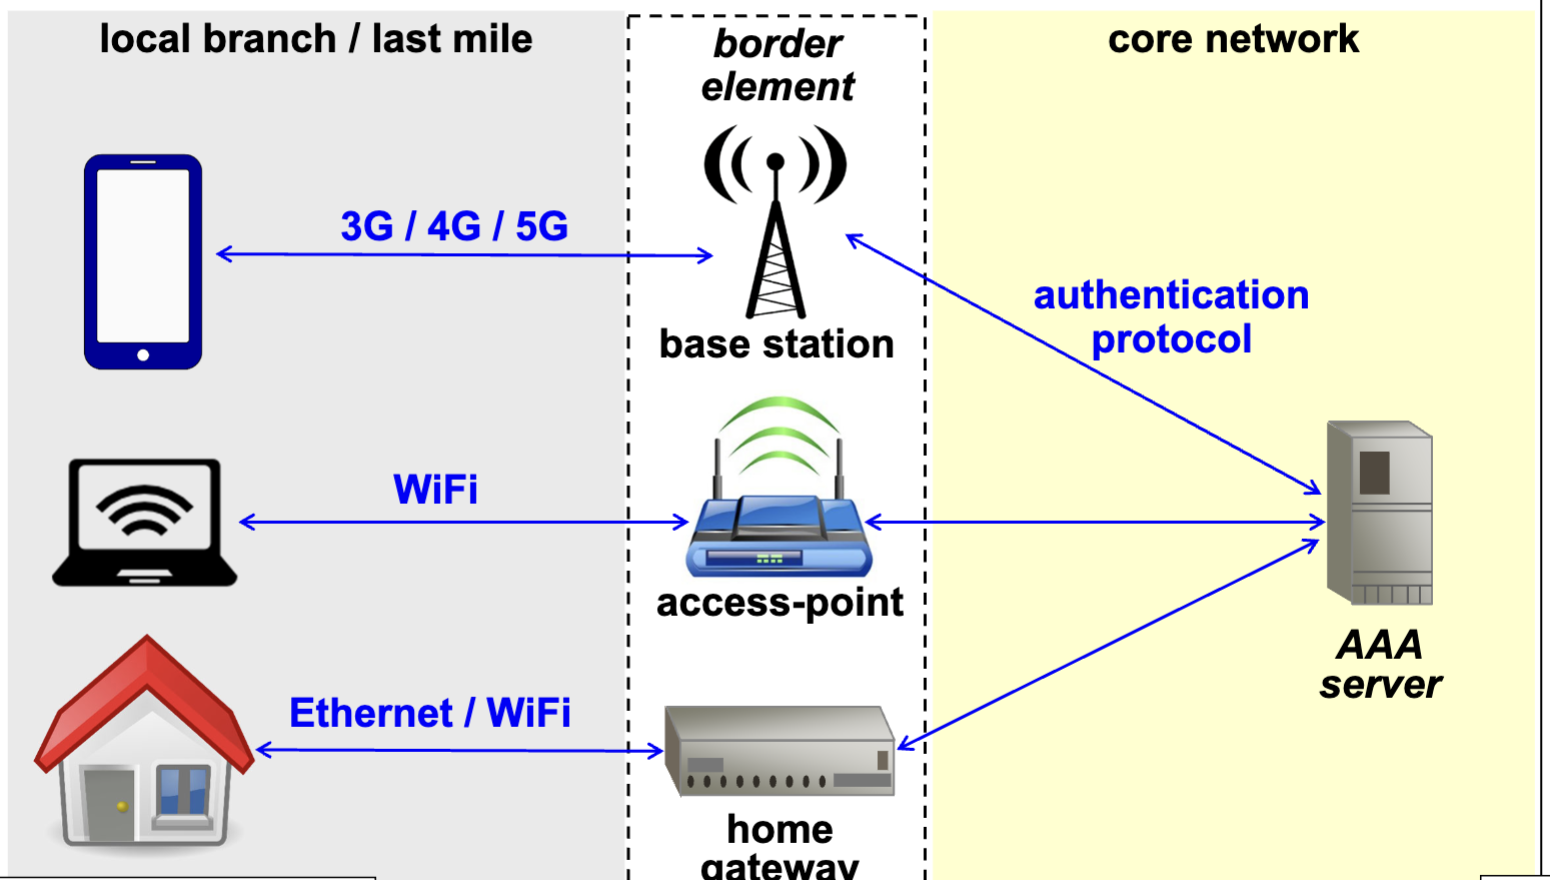
\includegraphics[width=\linewidth]{Images/NetSec/NetAccesModern.png}
        \caption{Net access, modern method}
    \end{figure}
\end{multicols}

\clearpage
\section{Point to Point Protocol}
\raggedright
    \begin{center}
        (PPP)
    \end{center}
The Point-to-Point Protocol (PPP) is a Data Link layer protocol (Layer 2 in the ISO/OSI stack) used for establishing direct connections between two network nodes. PPP is able to encapsulate network packets and carry them over a point-to-point link.

There are several types of links: \textbf{Physical} (legacy types, e.g., Public Switched Telephone Network (PSTN)), \textbf{Virtual Layer 2} (L2, e.g., Digital Subscriber Line (xDSL) with Point-to-Point Protocol over Ethernet (PPPoE)), and \textbf{Virtual Layer 3} (L3, e.g., Layer 2 Tunneling Protocol (L2TP) over UDP/IP).

A point-to-point link is activated in three sequential steps:
\begin{itemize}
    \item \textbf{Link Establishment}: The devices at both ends of the link establish a connection, usually through signaling or negotiation protocols (LCP - Link Control Protocol), such as PPP (Point-to-Point Protocol).
    \item \textbf{Authentication}: If necessary (\textcolor{red}{Optional!!}), authentication takes place to verify the identity of the connecting devices, often using protocols like Password Authentication Protocol (PAP), Challenge Handshake Protocol (CHAP) or Extensible Authentication Protocol(EAP) framework.
    \item \textbf{Network Layer Configuration}: Once the link is established and authenticated, L3 encapsulation is performed via various Network Control Protocols (NCPs), such as IP Control Protocol (IPCP) for IP packets, enabling data transfer to begin.
\end{itemize}

\section{Authentication at Data Link Layer}
\begin{center}
    For network access.

    After the link is established, optional authentication protocols are used to verify the identity of the connecting devices.
\end{center}
All the following protocols are used for authentication in network access scenarios, where a user or device must verify its identity before being granted access to a network or its resources. Using PPP as a reference, these protocols are employed during the authentication phase of a PPP connection.
\begin{tcolorbox}[colback=red!10!white, colframe=red!70!black, coltitle=white, title=Be aware]
    The following protocols are not exclusively used only for PPP.
\end{tcolorbox}

\subsection{Link Control Protocol Authentication Protocol}
\begin{center}
    (LCP Authentication Protocol)
\end{center}
LCP is responsible for \textbf{negotiating} various options, including those related to authentication. The LCP Authentication Protocol allows two devices at either end of the PPP link to agree on which authentication protocol to use (if any) for the connection. This option is part of the LCP negotiation phase. 

\clearpage
\textbf{Structure of the configuration option:}
\begin{itemize}
    \item Type (8 bits): This field defines the option type, indicating that it is an authentication protocol option. A value of 3 indicates that the authentication protocol is being negotiated.
    \item Length (8 bits): This field indicates the length of the option in bytes, including the type, length, protocol identifier, and any additional data.
    \item Authentication protocol (16 bits): Protocol identifier (For PAP is 0xC023 and CHAP is 0xC223).
    \item Algorithm (8 bits): Algorithm identifier (\textcolor{red}{Optional!!}). Used when the protocol supports multiple algorithms
\end{itemize}

\subsection{Password Authentication Protocol}
\begin{center}
    (PAP - RFC 1334 - Obsolete)
\end{center}
The key features are: 
\begin{itemize}
    \item ID and PWD are sent in clear text.
    \item Use of an Identifier to match Request and Response and prevent (partially) from replay attacks.
\end{itemize}

\subsubsection*{2-Way Handshake}

\begin{tcolorbox}[colback=yellow!10!white, colframe=yellow!70!black, title=Peer \textrightarrow Authenticator] 
    
    \begin{itemize}
        \item \underline{Authenticate Request} (code=1)
        \item Packet structure:
        \begin{itemize}
            \item Code (8 bits) + Identifier (8) + Length (16)
            \item Peer-ID-Length (8) + Peer-ID (0-255 B)
            \item Passwd-Length (8) + Passwd (0-255 B)
        \end{itemize}
    \end{itemize}
\end{tcolorbox}

\begin{tcolorbox}[colback=yellow!10!white, colframe=yellow!70!black, title=Authenticator \textrightarrow Peer] 
    
    \begin{itemize}
        \item \underline{Authenticate Response} (code= either 2 or 3)
        \begin{itemize}
            \item 2 stands for Acknowledgment (ACK)
            \item 3 stands for Negative Acknowledgment (NAK)
        \end{itemize}
        \item Packet structure:
        \begin{itemize}
            \item Code (8 bits) + Identifier (8) + Length (16)
            \item Message-Length (8) + Message (0-255 B)
        \end{itemize}
    \end{itemize}
\end{tcolorbox}


\subsection{Challenge Handshake Authentication Protocol}
\begin{center}
    (CHAP - Obsolete)

    Based on a CRA (Challenge-Response Authentication) model.
\end{center}

The key features are: 
\begin{itemize}
    \item Compulsory challenge at channel creation: The authenticator sends a challenge to the client. The client responds with a MAC (Message Authentication, and Integrity, Code - maybe keyed-digest), ensuring secure authentication (and integrity). Challenge or Response may be lost, so authenticator \underline{must} resend Challenge if no Response.
    \item Password are not sent in clear.
    \item The Authenticators that support both PAP and CHAP must offer CHAP first.
    \item Use of an Identifier to match Request and Response and prevent (partially) from replay attacks.
\end{itemize}

\subsubsection*{3-Way Handshake}


\begin{tcolorbox}[colback=yellow!10!white, colframe=yellow!70!black, title=Authenticator \textrightarrow Peer] 
    
    \begin{itemize}
        \item \underline{Challenge} (code=1)
        \item Packet structure:
        \begin{itemize}
            \item Code (8 bits) + Identifier (8) + Length (16)
            \item Challenge-Size (8) + Challenge-Value (0-255 B)
        \end{itemize}
    \end{itemize}
\end{tcolorbox}


\begin{tcolorbox}[colback=yellow!10!white, colframe=yellow!70!black, title=Peer \textrightarrow Authenticator] 
    
    \begin{itemize}
        \item \underline{Response} (code=2)
        \item Packet structure:
        \begin{itemize}
            \item Code (8 bits) + Identifier (8) + Length (16)
            \item Response-Size (8) + Response-Value (0-255 B)
        \end{itemize}
        \item Response-Value = md5 (Identifier || password || Challenge)=MAC
    \end{itemize}
\end{tcolorbox}




\begin{tcolorbox}[colback=yellow!10!white, colframe=yellow!70!black, title=Authenticator \textrightarrow Peer] 
    
    \begin{itemize}
        \item \underline{Authenticate Response} (code= either 3 or 4)
        \begin{itemize}
            \item 3 stands for Acknowledgment (ACK)
            \item 4 stands for Negative Acknowledgment (NAK)
        \end{itemize}
        \item Packet structure:
        \begin{itemize}
            \item Code (8 bits) + Identifier (8) + Length (16)
        \end{itemize}
    \end{itemize}
\end{tcolorbox}

\clearpage
\subsection{Microsoft Challenge Handshake Protocol}
\begin{center}
    (MS-CHAP - Obsolete)
\end{center}

MS-CHAP is a variant of CHAP designed by Microsoft, with two versions: MS-CHAP v1 and MS-CHAP v2. While these protocols share similar principles, they are \underline{distinct} and different from each other.

LCP negotiates CHAP algorithm: 0x80 for v1 and 0x82 for v2.

Key features in common (v1 and v2):
\begin{itemize}
    \item Authenticator-controlled password change.
    \item Authenticator-controlled authentication retry.
    \item Specific failure codes.
\end{itemize}

\subsection{MS-CHAP v2}
\begin{center}
    Insecure and obsolete for modern security standards due \newline to several significant vulnerabilities(Dictionary Attack\footnote{See Appendix A}).
\end{center}
\begin{itemize}
    \item Provides mutual authentication\footnote{Both the client and the server (authenticator) verify each other's identities during the authentication process} by piggybacking\footnote{The practice of sending additional data or control information within an existing communication, avoiding a separate or additional transmission} a peer challenge on the Response packet and including an authenticator response on the Success packet, which enables the client to verify the server's authenticity.
    \item Both peers (client and server) must have access to either the plaintext password or an MD4 hash of the password for the authentication to succeed. This requirement limits compatibility with password storage formats that do not support MD4 hashing or plaintext retrieval.
\end{itemize}

\begin{center}
    \textbf{The Protocol}
\end{center}
\begin{tcolorbox}[colback=yellow!10!white, colframe=yellow!70!black, title=Peer \textrightarrow Authenticator] 
    
    \begin{itemize}
        \item \underline{Initial Message} (*Hello*)
    \end{itemize}
    
\end{tcolorbox}

\textbf{Mutual AuthN:}
\begin{tcolorbox}[colback=yellow!10!white, colframe=yellow!70!black, title=Authenticator \textrightarrow Peer] 
    
    \begin{itemize}
        \item \underline{Server Challenge} - SC.
        \item Sending a 16-byte challenge generated by the authenticator.
    \end{itemize}
    
\end{tcolorbox}

\begin{tcolorbox}[colback=yellow!10!white, colframe=yellow!70!black, title=Peer \textrightarrow Authenticator] 
    
    \begin{itemize}
        \item \underline{Client Response} - H + R + username.
        \item H (Challenge Hash) is a condensed representation of the challenges and the username.
        \begin{itemize}
            \item H=sha1(SC||CC||username) [0, ..., 7].
        \begin{itemize}
            \item The Client Challenge (CC) is a 16-byte value generated by the Peer.
        \end{itemize}
        \item \textcolor{red}{Be aware: }Instead of using the full output of the SHA-1 hash (160 bits), it only takes the first 8 bytes of the result. 
        \end{itemize}
        
        \item R (Challenge-Response) = R1 || R2 || R3
        \begin{itemize}
            \item K (NT-Hash) is the MD4 hash of the password.
        \begin{itemize}
            \item K=md4 (password) \textcolor{Blue}{(128 bits digest)}.
        \end{itemize}
            \item R1 = DES(K[0,...,6], H) \textcolor{Blue}{(7 bytes)}
            \item R2 = DES(K[7,...,13], H).
            \item R3 = DES(K[14,...,20], H).
            \item \textcolor{red}{Be aware: } K has 16 bytes so, R's last 5 bytes are padded with 0's.
        \end{itemize}
    \end{itemize}
    
\end{tcolorbox}

\begin{tcolorbox}[colback=yellow!10!white, colframe=yellow!70!black, title=Authenticator \textrightarrow Peer] 
    
    \begin{itemize}
        \item \underline{Authentication Response} - A.
        \item A = sha1 (D || H || M2).
        \begin{itemize}
            \item M2 is a constant string: "Magic server to client signing constant".
            \item D (Digest) = sha1 (NHH || R || M1)
            
            \begin{itemize}
                \item NHH (NT-Hash-Hash) = md4 (md4 (password)).
                \item M1 is a constant string: "Magic server to client signing constant".
            \end{itemize}
        \end{itemize}
        \item The authenticator decrypts R and verifies whether the result matches H.
    \end{itemize}
    
\end{tcolorbox}

\begin{tcolorbox}[colback=yellow!10!white, colframe=yellow!70!black, title=Peer] 
    
    \begin{itemize}
        \item \underline{Client Checks}
        \item Peer computes A' and verifies whether it matches A.
        \begin{itemize}
            \item A' is the calculated authentication response by the client, which is computed in the same manner as A
        \end{itemize}
    \end{itemize}
    
\end{tcolorbox}

\clearpage 
\subsection{Extensible Authentication Protocol}
\begin{center}
    (EAP - Most adopted, but it's a \textcolor{red}{framework}).

    Supplicant-NAS communication.

    Encapsulation of frames + default authentication methods.
\end{center}

Key features:
\begin{itemize}
    \item Flexible L2 authentication framework.
    \item Uses predefined (\textcolor{blue}{default implementation}) mechanisms for authentication
    \begin{itemize}
        \item MD5-Challenge (similar to CHAP).
        \item One Time Password (OTP).
        \item Generic Token Card: Physical or virtual devices that generate a unique code or cryptographic key at regular intervals.
    \end{itemize}
    \item Other authentication mechanisms may be added: 
    \begin{itemize}
        \item PPP EAP TLS authentication protocol.
        \item RADIUS support for EAP.
    \end{itemize}
    \item EAP methods must provide security on their own (\textcolor{red}{Assumption: insecure link}).
\end{itemize}

\subsubsection*{EAP Encapsulation}

Authentication data are transported via a specific EAP encapsulation protocol (L3 packets are not yet available).

Encapsulation features:
\begin{itemize}
    \item Independent of IP (\textcolor{Blue}{operating at the data link layer of the stack}); in fact, supports any data link layer protocol.
    \item Explicit ACK/NAK (\textcolor{Blue}{no windowing}).
    \item Assumes no reordering.
    \begin{itemize}
        \item PPP guarantees ordering.
        \item UDP and raw IP not guarantee management of out-of-order packets.
    \end{itemize}
    \item Retransmission (max 3-5 retransmissions)
    \item No fragmentation (\textcolor{red}{must be provided by EAP methods for a payload greater than the minimum EAP Maximum Transfer Unit (MTU)})
\end{itemize}

\subsubsection*{EAP methods}

\begin{itemize}
    \item EAP-TLS (TLS mutual authentication).
    \item EAP-MD5 (only EAP client authentication).
    \item EAP-TTLS (Tunneled TLS): Operate any authentication method protected by TLS, e.g. PAP or CHAP.
    \item PEAP: TLS tunnel to protect and EAP method.
    \item EAP-SRP (EAP with Secure Remote Password).
    \item GSS\_API (includes Kerberos).
    \item AKA-SIM: Authentication and Key Agreement - Subscriber Identity Module. It is an authentication protocol used in mobile networks, specifically in 3G, 4G, and 5G systems.
\end{itemize}

\subsubsection*{EAP Architecture}

\begin{figure}[H]
    \centering
    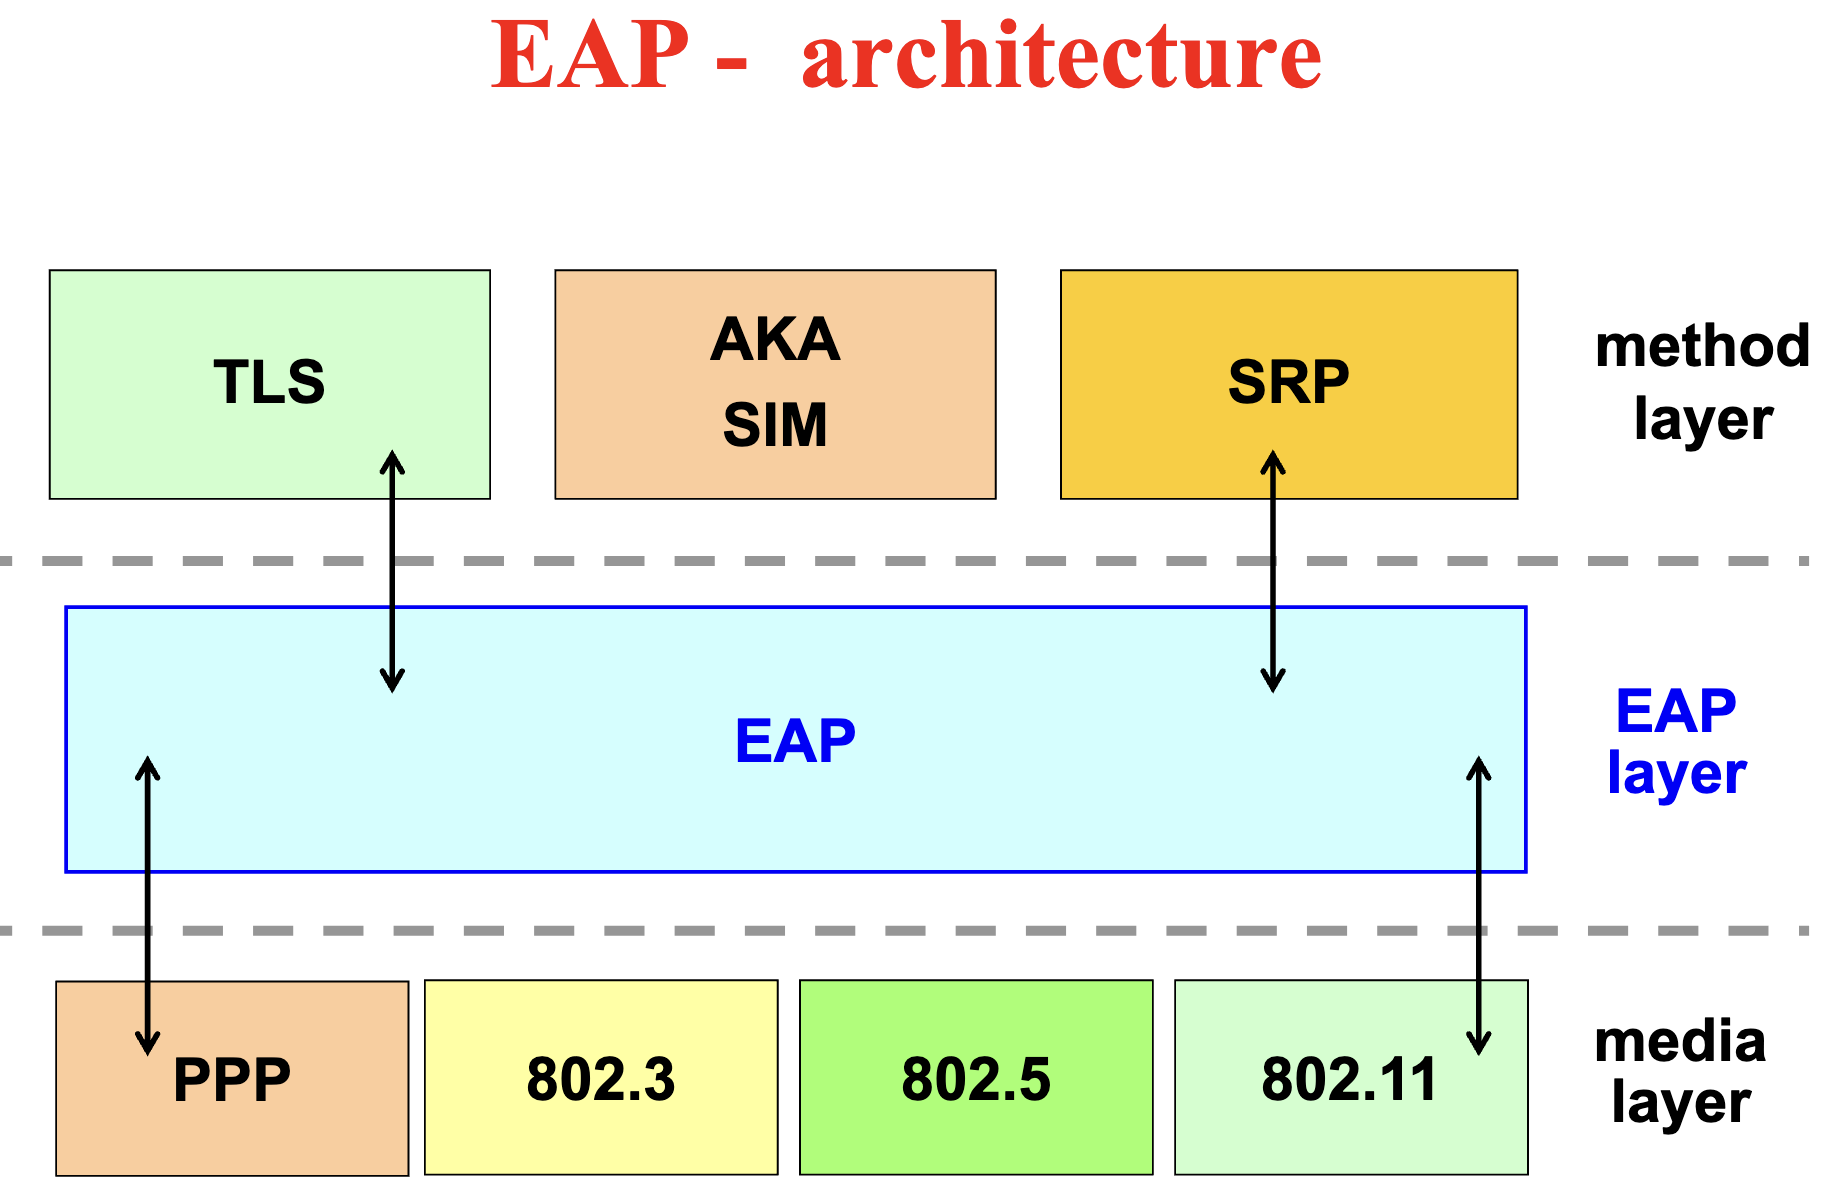
\includegraphics[width=0.5\linewidth]{Images/NetSec/eapArchitecture.png}
    \caption{Architecture of EAP}
\end{figure}

\begin{tcolorbox}[colback=blue!10!white, colframe=blue!50!white, title=Essentials of link-layer protocols] 
PPP \textrightarrow Point-to-Point Protocol

802.3 \textrightarrow Ethernet

802.5 \textrightarrow Token Ring

802.11 \textrightarrow Wi-Fi
\end{tcolorbox}

\section{Centralized Authentication for Network Access}
This diagram \ref{fig:network_authentication} illustrates the process of authenticating users for network access, involving multiple components to manage and verify permissions. 

Analyzing the main components:

\begin{multicols}{2}
    \raggedcolumns

    \begin{itemize}
        \item Network Access Server (NAS): This component serves as the entry point for devices attempting to connect to the network. The NAS collects credentials from users and initiates the authentication process.
        \item Protocol Manager: Acting as an intermediary, the protocol manager handles communication between the NAS and the Authentication Server.
\end{itemize}

\columnbreak

\begin{figure}[H]
    \centering
    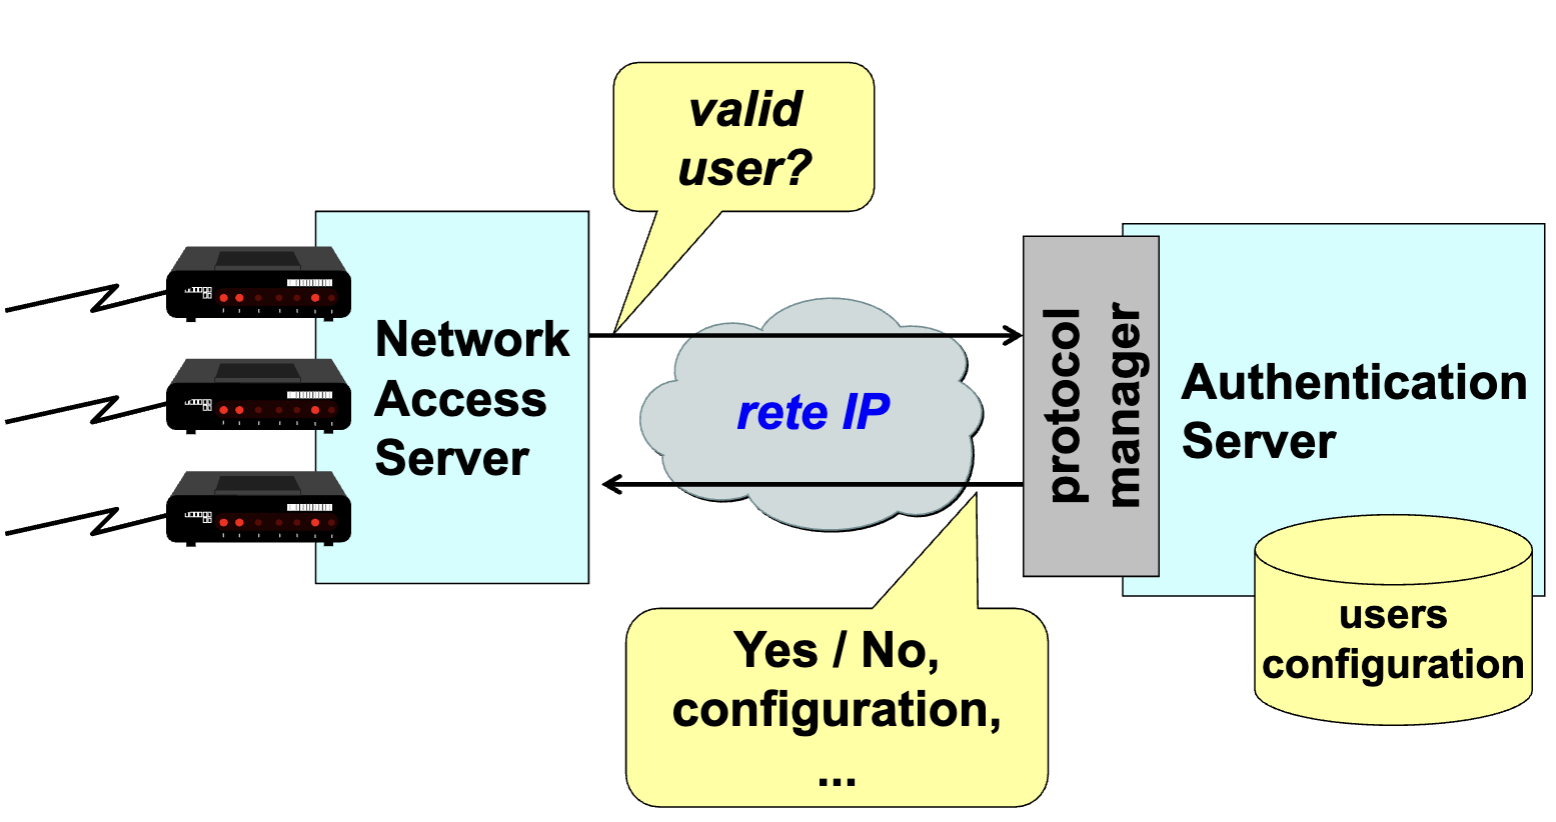
\includegraphics[width=\linewidth]{Images/NetSec/netsecConclusion.png}
    \caption{Authentication Mechanism for Complex Network Access}
    \label{fig:network_authentication}
\end{figure}
\end{multicols}
\begin{itemize}
    \item Authentication Server: The server verifies user credentials. It checks against a database (indicated as \texttt{users configuration} DB), which contains information about each user's permissions, restrictions, \boxed{and} allowed configurations (DHCP is no longer needed, also the connection speed is given!).
\end{itemize}



\begin{tcolorbox}[colback=red!10!white, colframe=red!70!black, coltitle=white, title=Beware]
In a large network, there are many NAS devices, each connected to a different network segment. So, the Authentication mechanism must be handled by a centralized server\dots
\end{tcolorbox}
\subsection{AuthN - AuthZ - AuthC Server}
\begin{center}
    (Crucial components of network security and access control.) \newline
    AAA Server strategy.
\end{center}

Network Access Server (NAS) manufacturers claim that Authentication Server's security needs three main functions:
\begin{itemize}
    \item Authentication: Verifying the identity of a user or device, ensuring that they are who they claim to be. Based on credentials.
    \item Authorization: Determining what an authenticated user or device is allowed to do within the network or system.
    \item Accounting: Tracking and logging the activities of users or devices on the network for auditing, monitoring, and reporting purposes.
\end{itemize}
The Authentication Server (AS) performs exactly these three functions, communicating with one or more Network Access Servers (NAS) via one or more protocols. 

Some of these protocols are:
\begin{itemize}
    \item RADIUS: Explained in the next section.
    \item DIAMETER: An evolution of RADIUS, designed to address its limitations and provide enhanced functionality (Especially regarding the security aspect.). Emphasis on roaming among different ISPs (proxy).
    \item TACACS+: Technically better than Radius, but less used because of its proprietary nature (Cisco).
\end{itemize}

\clearpage

\section{Remote Authentication Dial-In User Service}
\begin{center}
    (RADIUS - de facto standard for centralized network access control)

    NAS-AuthenticationServer communication protocol.
\end{center}
Protocol used for enabling a centralized authentication, authorization, and accounting (AAA) management for users who connect and use a network service.

Key features:
\begin{itemize}
    \item Is used for communication between a NAS and a backend Authentication Server (AS).
    \item Can also interconnect many authentication servers, acting as a \textbf{proxy server}.  
    \item Supports multiple authentication protocols, such as PAP, CHAP, and EAP.
    \item Relatively low security compared to modern protocols:
    \begin{itemize}
        \item Passwords obfuscation (not encryption).
        \item Passwords may be transmitted using less secure methods (e.g., PAP).
    \end{itemize}
    \item Operates over UDP (default ports: 1812 for authentication and 1813 for accounting).
    \item Widely used for remote access, VPNs, and enterprise Wi-Fi networks.
\end{itemize}

Security Properties:
\begin{itemize}
    \item Data Authentication of requests (request authenticator).
    \item Data Authentication/integrity and anti-replay of responses (response authenticator).
\end{itemize}


\subsection{RADIUS as Proxy Server}

\begin{multicols}{2}
\raggedcolumns
    The RADIUS server may act as a proxy \footnote{A proxy server intercepts and forwards requests} towards other authentication servers.
    The figure \ref{fig:RADIUS_proxy} depicts the RADIUS server forwarding each request as needed; the two company servers must have an agreement with the RADIUS server to handle authentication and authorization requests effectively.
    
    The address of NAS1 is \textcolor{red}{not an email address}; it is an identifier in the form: \texttt{user@authN\_domain}.
\columnbreak

\begin{figure}[H]
    \centering
    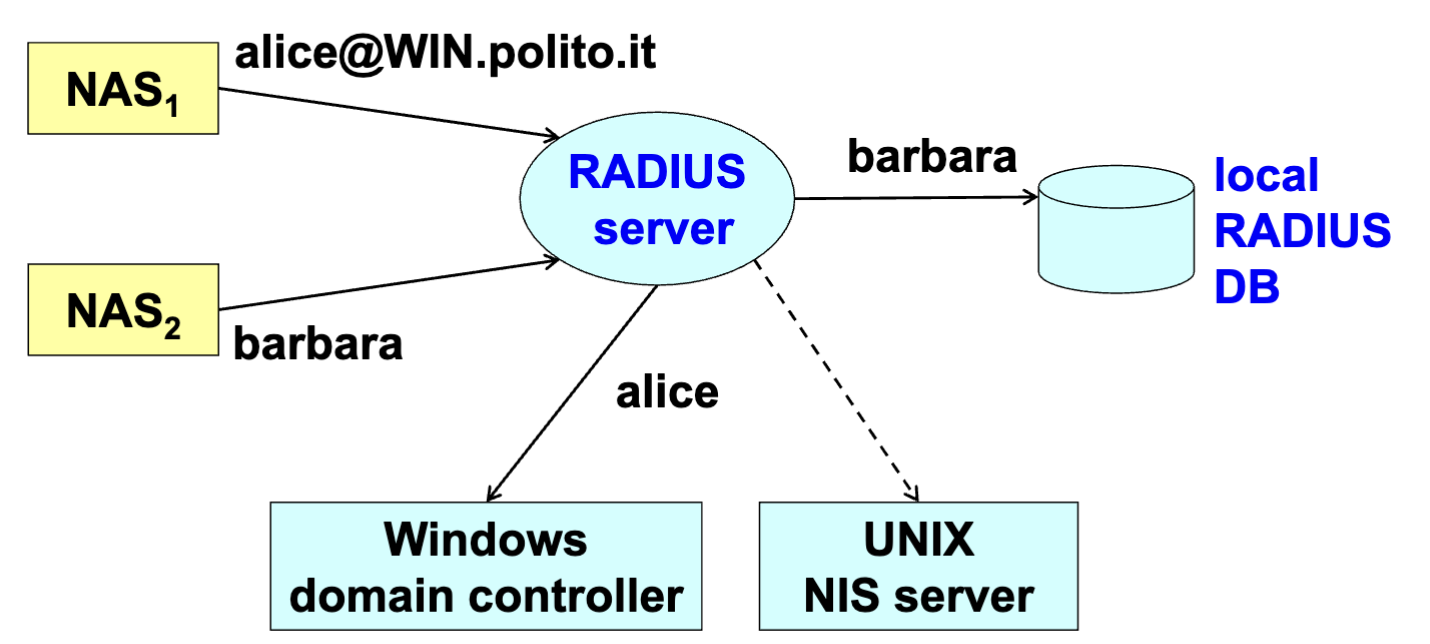
\includegraphics[width=\linewidth]{Images/NetSec/radiusProxy.png}
    \caption{RADIUS acting as a proxy server.}
    \label{fig:RADIUS_proxy}
\end{figure}
\end{multicols}




\subsection*{RADIUS Data Protection}
\begin{center}
    NAS (Network Access Server) and AS (Authentication Server) have a shared secret key.
\end{center}
RADIUS and NAS use MACs (keyed-digests, md5 or SHA-1) to ensure both the integrity and authenticity of the communication. If the MAC received and computed locally are not valid, the packet is discarded.

\begin{itemize}
    \item Password obfuscation formula: 
    \begin{equation*}
        \text{password} \oplus \text{MD5}(\text{key}\ ||\ \text{authenticator})
    \end{equation*}
    
    The password is padded with $0x00$ bytes (null bytes) so that its length becomes a multiple of 128 bits (16 bytes). This ensures the correct size for MD5 hashing, which operates on 128-bit blocks.

    \vspace{0.2cm}

    The authenticator serves a crucial role in ensuring both the authentication of the server's reply and the \underline{prevention of replay attacks}. It also helps in masking sensitive information like passwords (salting the password in order to reuse them).
\end{itemize}


The authenticator parameter:
\begin{itemize}
    \item In the \texttt{ACCESS-REQUEST} message Is named Request Authenticator and is a 16-byte value randomly generated by the NAS.
    \item In the \texttt{ACCESS-ACCEPT | REJECT | CHALLENGE} message Is named Response Authenticator and is computed via a keyed-digest.
    \begin{itemize}
        \item Response Authenticator formula:
        \begin{equation*}
            \text{MD5}(\text{code} \| \text{ID} \| \text{length} \|\text{Request Authenticator} \| \text{attributes} \| \text{secret})
        \end{equation*}
    \end{itemize}
\end{itemize}

\begin{figure}[H]
    \centering
    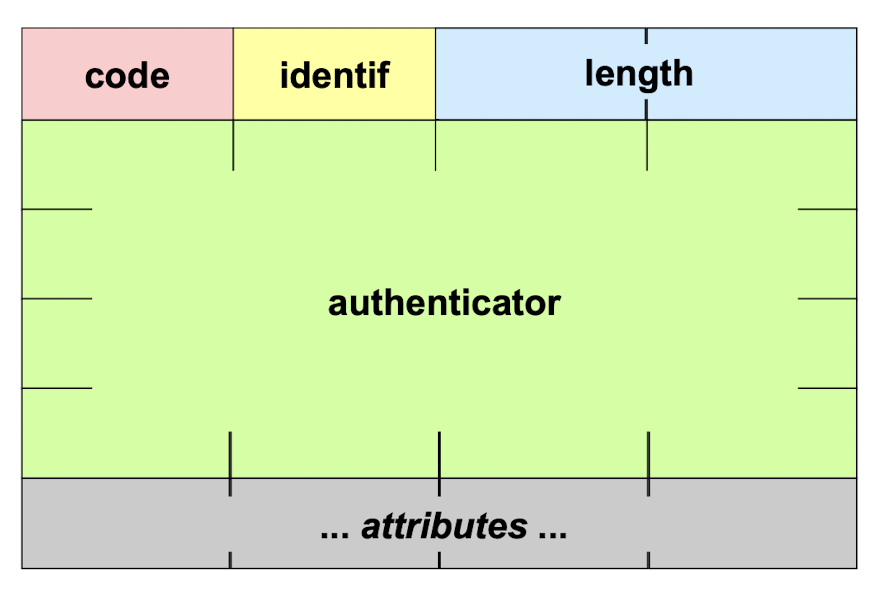
\includegraphics[width=0.5\linewidth]{Images/NetSec/radius_packet_format.png}
    \caption{RADIUS packet format.}
    
\end{figure}

\clearpage




\begin{tcolorbox}[colback=red!10!white, colframe=red!70!black, coltitle=white, title=Be aware] 
The username is the one used in the PPP authentication phase, does not necessarily match the application username.
\end{tcolorbox}
When a user attempts to connect to a Wi-Fi network or VPN, they might submit their credentials in the form username@domain.com (which is not an email address, but the identifier).



\subsubsection{RADIUS Attributes}
Possible Attributes:
\begin{itemize}
    \item 1 for User-Name (text), the \texttt{value} includes a Network Access Identifier (NAI - e.g. value= "alice" or "alice@domain.com") or a Distinguished Name\footnote{Is typically composed of several relative distinguished names (RDNs), which represent different attributes of the object, and they are arranged in a hierarchy, starting from the most specific to the most general. e.g. DN = CN=John Doe, OU=Users, DC=example, DC=com} (DN).
    \item 2 for User-Password (obfuscated password).
    \begin{equation*}
        \texttt{value} =password \oplus MD5(key\ \| \ RequestAuthenticator)
    \end{equation*}
    \item 3 for CHAP-Password (128-bit value).
    \begin{equation*}
        \texttt{value}=\text{user CHAP response}
    \end{equation*}
    \item 60 for CHAP-Challenge.
    \begin{equation*}
        \texttt{value}=\text{challenge from NAS \textrightarrow User}
    \end{equation*}
\end{itemize}


\subsubsection{RADIUS-NAS Packet Types}
There are different messages exchanged between the Network Access Server (NAS) and the RADIUS server.

\begin{itemize}
    \item ACCESS-REQUEST \textcolor{blue}{NAS \textrightarrow RADIUS}: Contains the access credentials provided by the user, such as the username and password.
    \item ACCESS-CHALLENGE \textcolor{Blue}{RADIUS \textrightarrow NAS}: Requests additional data, such as a PIN, token code, or a secondary password, in case multifactor authentication (MFA) is enabled.
    \item ACCESS-REJECT \textcolor{Blue}{RADIUS \textrightarrow NAS}: Includes a reason for denial, such as an incorrect username or password, or the user not having sufficient permissions.
    \item ACCESS-ACCEPT \textcolor{Blue}{RADIUS \textrightarrow NAS}: Includes network parameters or attributes that define the user's network access permissions.
\end{itemize}
\clearpage

\subsection{Example}
\begin{center}
    Using CHAP as authentication protocol.
\end{center}
The figure \ref{fig:chap_plus_radius} illustrates the interaction between CLIENT, NAS and RADIUS for authenticating users in a network access scenario. 


    \textbf{Key points:}
\begin{enumerate}
    \item The NAS (Network Access Server) initiates the authentication process by sending a Challenge Request. This step is necessary due to the use of CHAP (Challenge Handshake Authentication Protocol).
    \item To verify the credentials (contained in the \texttt{Challenge\_Response} message), the NAS forwards the authentication request to the RADIUS server. The RADIUS server acts as the central verifier, ensuring that the provided credentials are correct.
    \item The RADIUS server processes the request and returns a response:
    \begin{itemize}
        \item If the credentials are valid, the RADIUS server responds with an \texttt{Access-Accept} message, providing allowed configurations (such as IP address, DNS settings, etc.). 
        \item If the credentials are invalid, the server sends an \texttt{Access-Reject} message.
    \end{itemize}
        \item The NAS forwards the RADIUS server's response to the client, allowing or denying access based on the server's decision.
    \end{enumerate} 
    
   

    \begin{figure}[H]
        \centering
        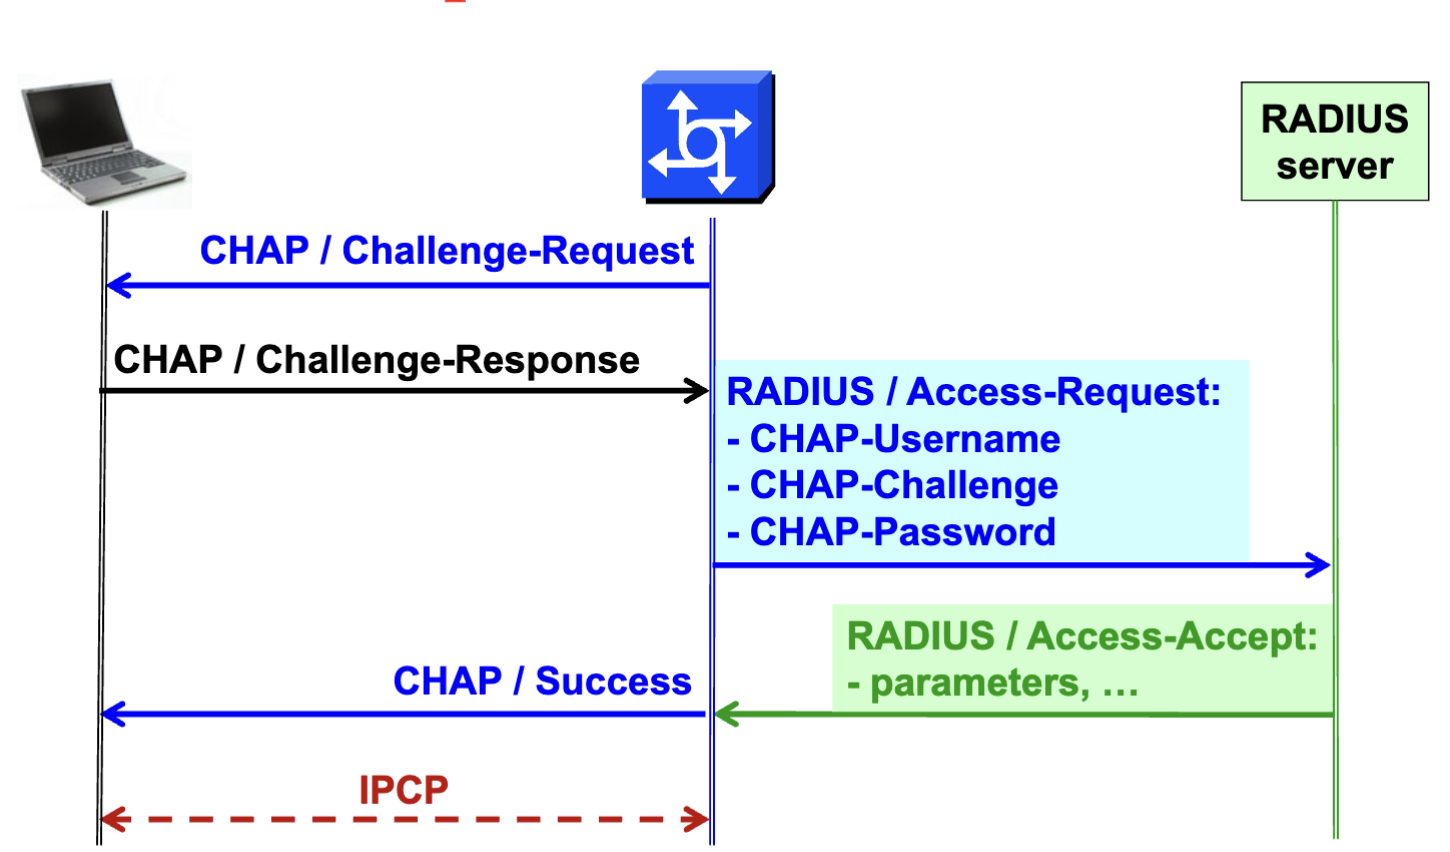
\includegraphics[width=0.7\linewidth]{Images/NetSec/chap_plus_radius.png}
        \caption{Example of CHAP + RADIUS.}
        \label{fig:chap_plus_radius}
    \end{figure}



\clearpage

\subsection{IEEE 802.1x}
\begin{center}
    Port-Based Network Access Control.
\end{center}

Key features:
\begin{itemize}
    \item L2 authentication mechanism.
    \begin{itemize}
        \item Session keys may be derived for use in packet authentication, integrity, and confidentiality (use of Standard algorithms for key derivation, e.g., TLS, SRP).
    \end{itemize}
    \item For authentication are used EAP-based protocols.
    \begin{tcolorbox}[colback=red!10!white, colframe=red!70!black, coltitle=white, title=Be aware] 
        EAP is a framework, not a specific authentication method, and it can support various authentication methods.
    \end{tcolorbox}
\end{itemize}

Other key points:
\begin{itemize}
    \item \textcolor{red}{Exploits the Application Layer for implementing security mechanisms\footnote{The detailed security operations (e.g., encryption, key management, etc.) are not directly handled at the lower layers (like the physical or data link layers). Instead, these mechanisms are implemented and operate at the application layer, which is responsible for initiating and managing the security processes.}.}
    \begin{itemize}
        \item Direct dialogue between supplicant and AS.
        \item As long as the devices support 802.1X, they don't need modification to implement new security mechanisms—it's handled by the authentication and key management processes at the application layer.
    \end{itemize}
    \item Useful in a wired network to block access.
\end{itemize}

\subsubsection*{IEEE 802.1x Architecture}
The architecture of IEEE 802.1X (in figure \ref{fig:8021x_architecture}) consists of three primary components that interact to provide network authentication. Here's an overview of these components:


\begin{multicols}{2}
\raggedcolumns
    \begin{itemize}
        \item Supplicant (Client Device): The device (e.g., a laptop, smartphone, or any client device) that requests access to the network.
        \item Authenticator:  Is usually a network switch, wireless access point (WAP), or another network access device (not a typical one). Doesn't authenticate the client itself; instead, it forwards the authentication requests to the authentication server (RADIUS server).
        \item Authentication server (AS): Typically implements RADIUS, performs the actual authentication of the supplicant. 
    \end{itemize}
\columnbreak

    
\begin{figure}[H]
    \centering
    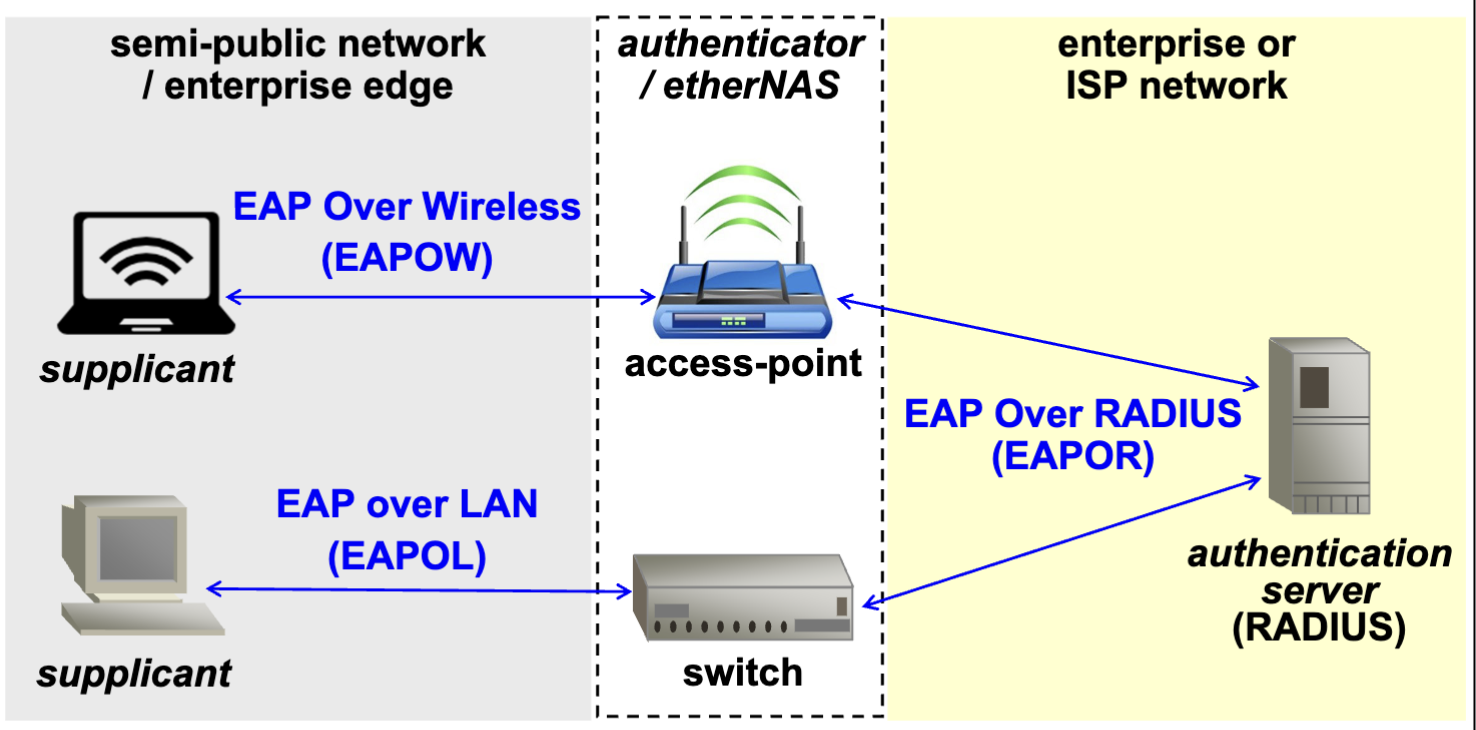
\includegraphics[width=\linewidth]{Images/NetSec/8021x_architecture.png}
    \caption{802.1x Architecture.}
    \label{fig:8021x_architecture}
\end{figure}
\end{multicols}

\subsubsection*{IEEE 802.1x Messages}
The diagram \ref{fig:8021.x_messages} illustrates the IEEE 802.1X authentication process using a switch as an authenticator and a RADIUS server as the authentication server.
On the left side, we have EAPOL (Extensible Authentication Protocol over LAN) messages, and on the right side, we have RADIUS messages.  The port initially blocks access until the authentication is completed.

\hfill 

\textbf{EAPOL (Extensible Authentication Protocol over LAN) Messages}:
\begin{itemize}
    \item EAPOL-Start: The client (laptop) sends an EAPOL-Start message to indicate it wants to begin the authentication process.
    \item The switch, acting as the authenticator (NAS), sends an EAP-Request/Identity message to the client to ask for its identity (ID).
    \item The client responds with an EAP-Response/Identity message containing its identity (ID).
    \item The switch forwards the client's authentication information to the RADIUS server in a Radius-Access-Request message.
    \item If additional verification is needed (like a PIN or token), the RADIUS server responds with a Radius-Access-Challenge. The switch forwards this to the client, and the client responds with additional credentials if required.
    \item The switch forwards the additional request for credentials to the client.
    \item The client provides the requested credentials in an EAP-Response message. This data is then relayed to the RADIUS server.
    \item Once the RADIUS server has validated the credentials, it replies with either a Radius-Access-Accept (if the client is authenticated) or a Radius-Access-Reject (if authentication fails).
\end{itemize}
If authentication is successful, the switch sends an EAP-Success message to the client, and network access is granted.
\begin{figure}[H]
    \centering
    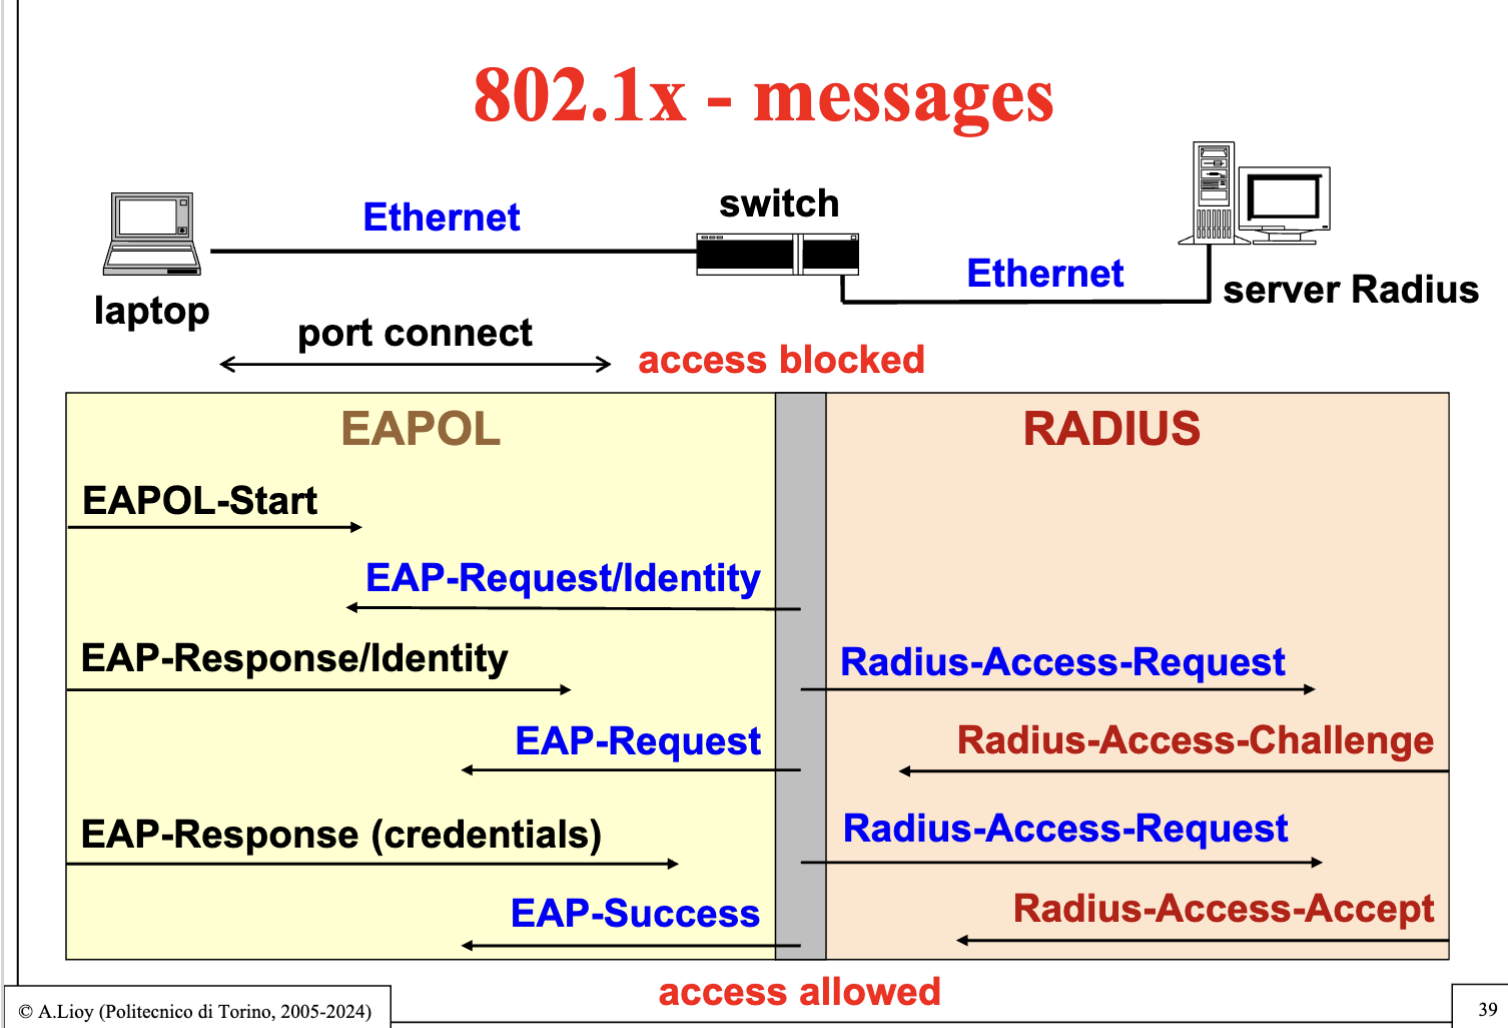
\includegraphics[width=0.5\linewidth]{Images/NetSec/8021x_messages.png}
    \caption{802.1x Messages.}
    \label{fig:8021.x_messages}
\end{figure}

\hfill
\begin{center}
    \boxed{\textbf{At Which Level Must we Implement Security?}}
\end{center}

\begin{center}
    Security must be implemented at multiple levels (\textcolor{Blue}{defense-in-depth approach}) to ensure comprehensive protection in any system or infrastructure.
\end{center}
\hfill 

There is no optimal level for implementing security; however, it is important to understand that the higher the level, the less general the information contained in the packets.

\begin{tcolorbox}[colback=lightblue, colframe=blue!50!white]
    Upper in the stack \textrightarrow More specific security functions.
    
    Lower in the stack \textrightarrow More general security functions.
\end{tcolorbox}

\section{Security at Layer 2 (ISO/OSI)}
\begin{center}
Data link layer in the OSI model
\end{center}
\begin{center}
    \subsection{DHCP Protection}
\end{center}

\begin{center}
    (Dynamic Host Configuration Protocol)
\end{center}
Protocol to provide hosts with IP addresses and other network configuration parameters.
(look slides netsec)

Best Practices for protecting Against DHCP Attacks:
\begin{itemize}
    \item Enable DHCP Snooping.
    \item Enable IP guard.
    \item Restrict Network Access (e.g. VLANs, IEEE 802.x).
\end{itemize}

\clearpage
\section{Security at Layer 3 (ISO/OSI)}
\begin{center}
(Network layer in the OSI model)
    
\end{center}
It focuses on securing the transmission of data between endpoints (\textcolor{Blue}{end-to-end protection}). For L3-homogeneous networks (e.g., IP networks), this requires defining real clients and servers, as external features are not visible.

Many solutions are listed below (like VPNs or IPsec).

\begin{center}
    \subsection{Virtual Private Networks}
\end{center}
\begin{center}
    (VPNs)
\end{center}

\textbf{Definition and Utility}:

\vspace{0.2cm}


\begin{multicols}{2}
\raggedcolumns
    VPNs are techniques (hardware or software) used to create a private network over shared or untrusted channels and transmission devices, ensuring secure communication between remote endpoints.

    The figure \ref{fig:vpn_definition} illustrates how a telecommunication company carries your private traffic separately from other private networks.
    
\columnbreak

\begin{figure}[H]
    \centering
    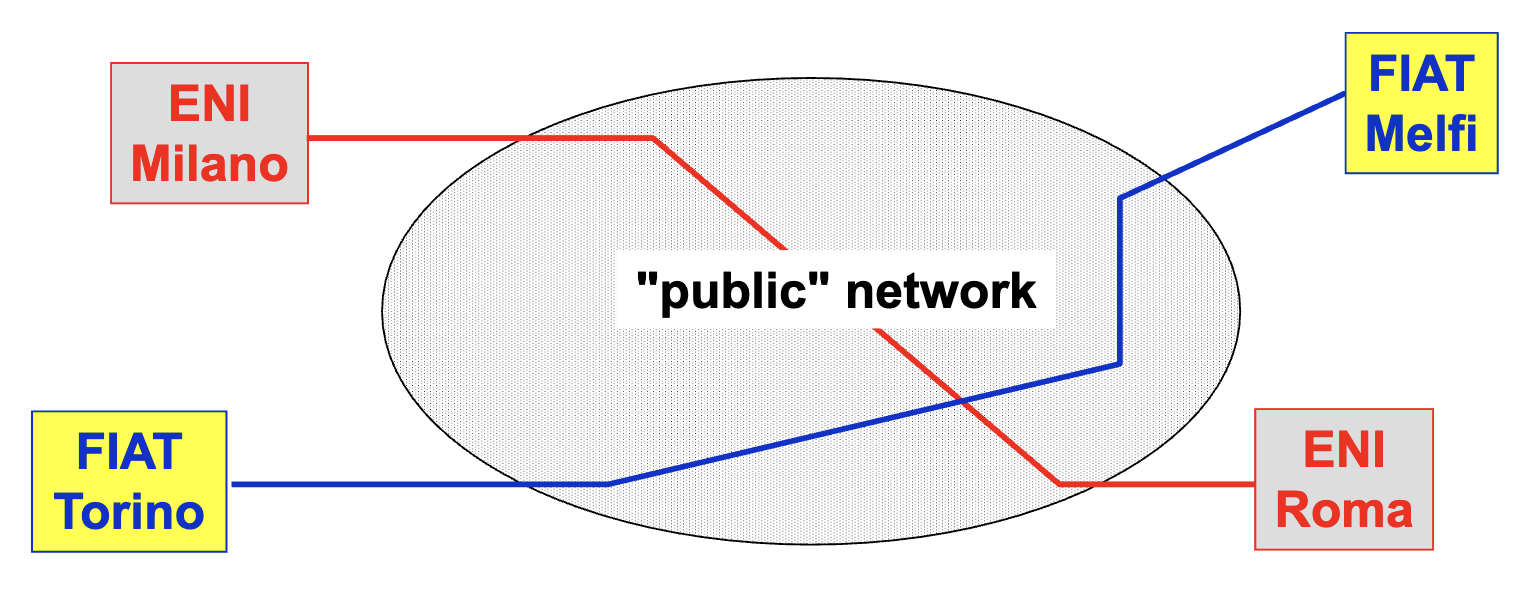
\includegraphics[width=\linewidth]{Images/NetSec/vpn_definition.png}
    \caption{VPN Example}
    \label{fig:vpn_definition}
    
\end{figure}
\end{multicols}

\textbf{Techniques to Create a VPN}

\vspace{0.2cm}

We must provide \underline{mutual} security for both actors.
\begin{itemize}
    \item User: Must be assured of confidentiality, integrity, and authenticity of their data while transmitted over the network.
    \item Provider: Must prevent unauthorized access to the network infrastructure.
\end{itemize}

Then we can analyze some techniques of VPN:
\begin{itemize}
    \item Via \textbf{private addressing}.
    \item Via \textbf{IP tunnel} (protected routing).
    \item Via \textbf{secure IP tunnel} (cryptographic protection of the network packets).
\end{itemize}
\begin{center}
    \subsubsection{VPN via Private Addresses}
\end{center}
Use of private IP address spaces\footnote{Private IANA networks RFC-1918.} (non-public addresses) to create a secure network tunnel between endpoints while keeping the actual IP addresses of the users or internal networks \underline{hidden or separated} from the public internet.


\begin{tcolorbox}[colback=red!10!white, colframe=red!70!black, coltitle=white, title=Be aware] 
0 security!! Poor solution.
\end{tcolorbox}

\clearpage
    \subsubsection{VPN via IP Tunnel}
\begin{center}
    (Protected Routing)

    \textcolor{red}{Security only for the network provider}
\end{center}


\begin{multicols}{2}
\raggedcolumns

    The routers encapsulate whole L3 packets as a payload inside another packet (e.g. IP in IP, IP over MPLS). The routers perform access control to the VPN by ACL (Access Control List).

    This protection can be easily defeated by anybody that manages a router or can sniff the packets during transmission.
\columnbreak

\begin{figure}[H]
    \centering
    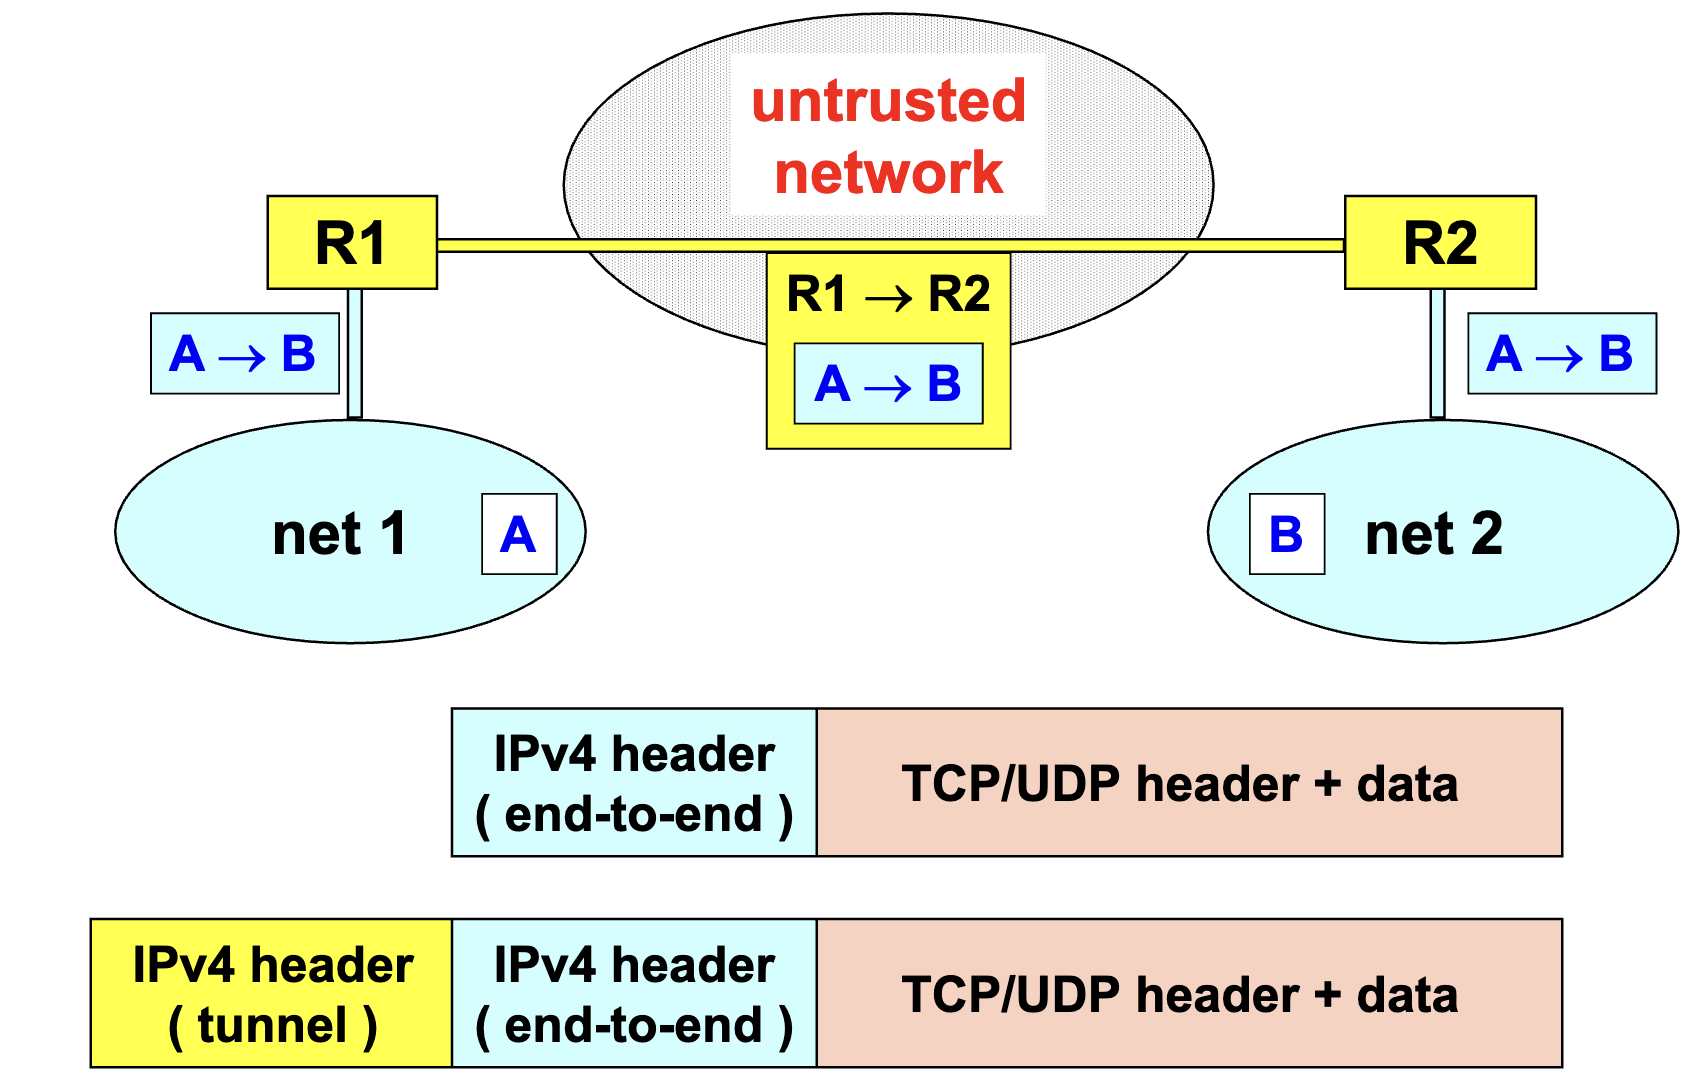
\includegraphics[width=\linewidth]{Images/NetSec/vpn_via_ip_tunnel.png}
    \caption{VPN via IP tunnel example.}    
\end{figure}
\end{multicols}


\subsubsection{VPN via Secure IP Tunnel}
\begin{center}
    (Cryptographic Protection of the Network Packets)
\end{center}
\begin{multicols}{2}

\raggedcolumns
    Before encapsulation (as seen above), the packets are protected with:
    \begin{itemize}
        \item \textcolor{Blue}{Integrity + AuthN} from MAC (Message Authentication Code).
        \item \textcolor{Blue}{Confidentiality} from Encryption.
        \item Partial-solution to avoid replay attacks from Numbering.
    \end{itemize}
\columnbreak

\begin{figure}[H]
    \centering
    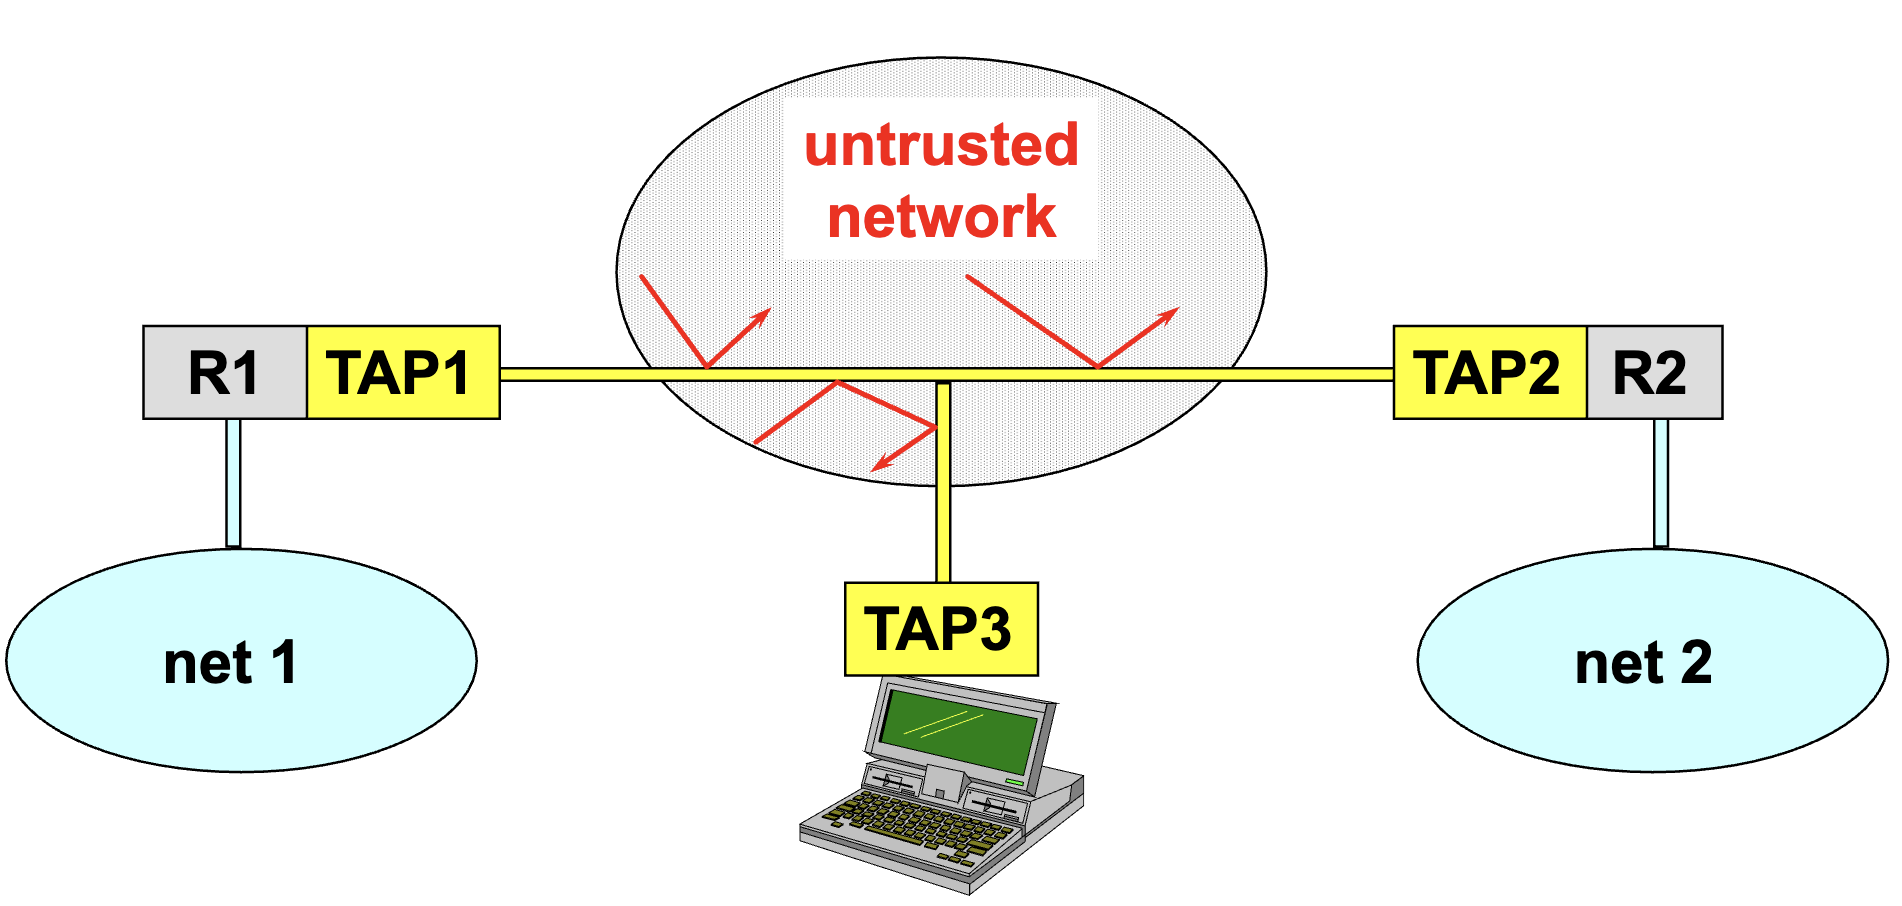
\includegraphics[width=\linewidth]{Images/NetSec/vpn_via_encrypt_tunnel.png}
    \caption{VPN via secure IP tunnel example.}    
\end{figure}
\end{multicols}






\begin{tcolorbox}[colback=blue!10!white, colframe=blue!50!white, title=How to Damage the Communication?] 
    If the cryptographic algorithms are strong, the only viable attack is to disrupt or stop the communication. However, a DOS attack is still possible.
\end{tcolorbox}



\begin{tcolorbox}[colback=red!10!white, colframe=red!70!black, coltitle=white, title=Be aware] 
    The TAP* should not be managed by the company that sells the VPN (or the network provider), as this could allow for potential manipulation.
\end{tcolorbox}

\clearpage
\begin{center}
    \section{IPsec}
\end{center}
IPSec (Internet Protocol Security) is a suite of protocols used to secure IP communications. Let create S-VPN (Secure Virtual Private Networks) over untrusted networks or to create end-to-end secure communication. 

\hfill

\begin{tcolorbox}[colback=blue!10!white, colframe=blue!50!white, title=Reminder] 
    Not all the traffic needs confidentiality.
\end{tcolorbox}

\hfill

\textbf{Packet Types:}
\begin{itemize}
    \item AH (Authentication Header): Integrity, AuthN and no replay to the entire packet.
    \item ESP (Encapsulating Security Payload): Confidentiality (and authentication if last version).
\end{itemize}

The protocol for key exchange is IKE (Internet Key Exchange), which is \textcolor{red}{independent of the IP address}.

\hfill 

\textbf{Security Services:}
\begin{itemize}
    \item \textcolor{Blue}{Data Authentication/Integrity}: Computation of a MAC  with a shared key (keyed-digest). 
    \item Partial protection \textcolor{Blue}{against replay} attacks: Sequence number for the packets (creation is mandatory for the server and verification is optional for the client).
    \item Data Confidentiality: Packet's payload encryption with a symmetric algorithm (use of a shared key) and Data Privacy.
    \item Peer Authentication when creating the SA (Security Association): The key agreement comes after authentication (pre-shared key or digital signature).
\end{itemize}

\subsection{IPsec Security Association}
\begin{center}
    (IPsec SA)
\end{center}
A unidirectional logical connection. Each Security Association (SA) is associated with different security services. At least two SAs are needed to provide complete protection for a bidirectional packet flow.

\begin{tcolorbox}[colback=lightblue] 
    Protection can be made in different ways, with each Security Association (SA) being associated with specific security services. For example, one SA might provide encryption for confidentiality, while another might provide authentication for data integrity and sender verification. 
\end{tcolorbox}


\begin{figure}[H]
    \centering
    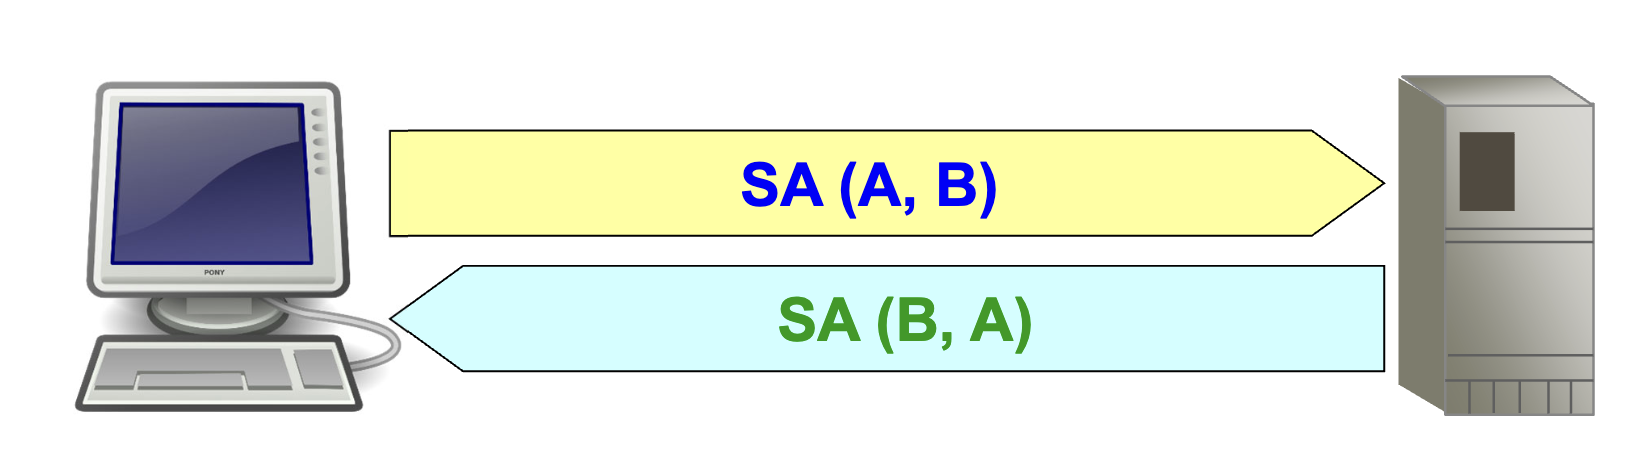
\includegraphics[width=0.5\linewidth]{Images/NetSec/SA.png}
    \caption{IPsec Security Association example.}
\end{figure}

\subsection{IPsec Local Database}

The IPsec Local Database is a crucial component in managing IPsec policies and associations. It consists of two main parts:

\begin{itemize}
    \item \textbf{Security Policy Database} (SPD)
    \begin{itemize}
        \item Contains a list of security policies that define how different packet flows should be handled.
        \item Can be a-priori configured (e.g., manually set by an administrator) or can be dynamically managed through an automatic system (such as an Internet Security Policy System (ISPS)).
        \item Each SPD entry corresponds to a traffic flow and specifies the corresponding security measures (e.g., encryption, authentication).
    \end{itemize}
    \item \textbf{Security Association Database} (SAD)
    \begin{itemize}
        \item Each entry in the SAD contains the characteristics of a specific SA (the specific agreement), including encryption algorithms, authentication keys, and other parameters needed to secure the communication.
    \end{itemize}
\end{itemize}

\subsection{IPsec Packet Sending}


    \begin{enumerate}
        \item Traffic Classification: The outgoing packet is checked against the rules in the Security Policy Database (SPD) to determine whether it needs IPsec protection, should bypass IPsec (direct link to layer 2), or be discarded.
        \item Security Association Lookup: If protection is required, the system consults the Security Association Database (SAD) to locate an active Security Association (SA) corresponding to the traffic flow.
        \item Applying Security Services: The appropriate security services are applied based on the SA:
        \begin{itemize}
            \item Authentication Header (AH): Adds integrity and authentication to the packet.
            \item Encapsulating Security Payload (ESP): Encrypts the payload for confidentiality and optionally provides authentication (in the newer versions).
        \end{itemize}
        \item Encapsulation, The packet is encapsulated depending on the IPsec's specific mode of operation: Transport Mode or Tunnel Mode.
    \end{enumerate}



\begin{figure}[H]
    \centering
    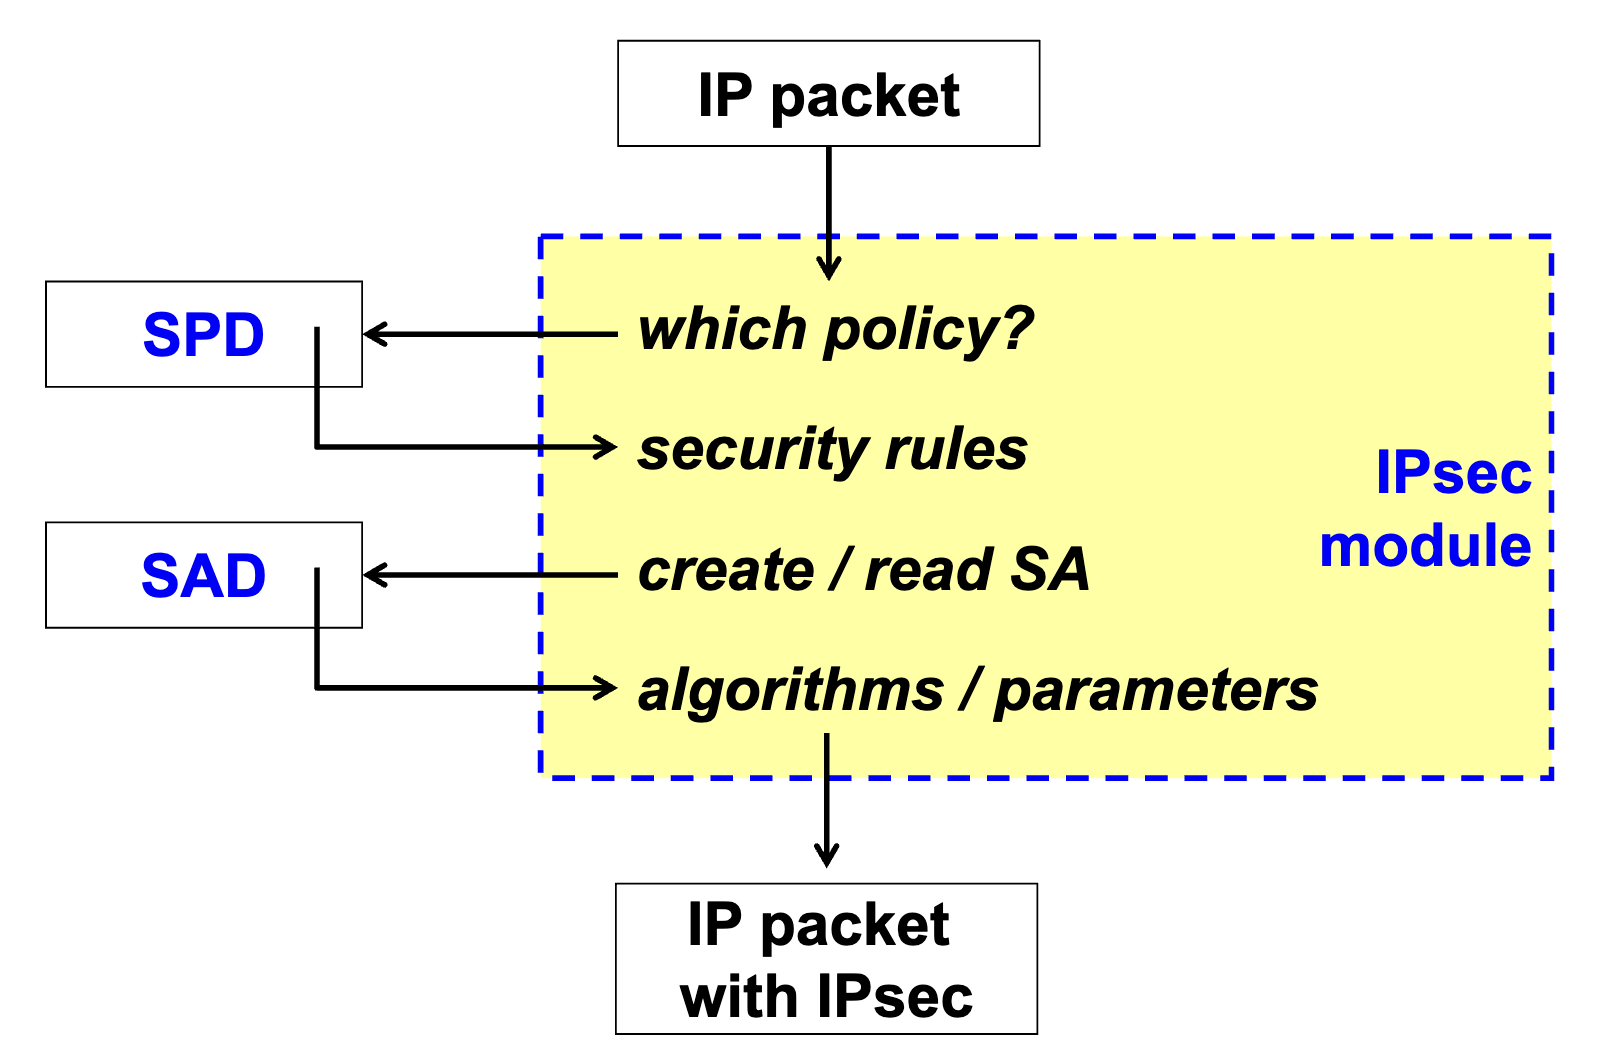
\includegraphics[width=0.3\linewidth]{Images/NetSec/ipsect_sending.png}
    \caption{How IPsec works (sending).}
    \label{fig:IPsec_packet_sending}
\end{figure}

\subsection{IPsec Transport mode}
\begin{center}
    Reduced encapsulation, computationally light.
\end{center}
Encapsulate the original IP packet within a new IP packet, providing protection for the original IP packet (except the variable fields of the header).

\begin{multicols}{2}
\raggedcolumns
    A key limitation is that the \textbf{variable fields} in the original IP \textbf{header}, such as the Time-to-Live (TTL) or checksum, remain exposed. This lack of protection can potentially be exploited, as attackers may analyze or manipulate these fields to gather information about the network or disrupt communication.

\columnbreak

\begin{figure}[H]
    \centering
    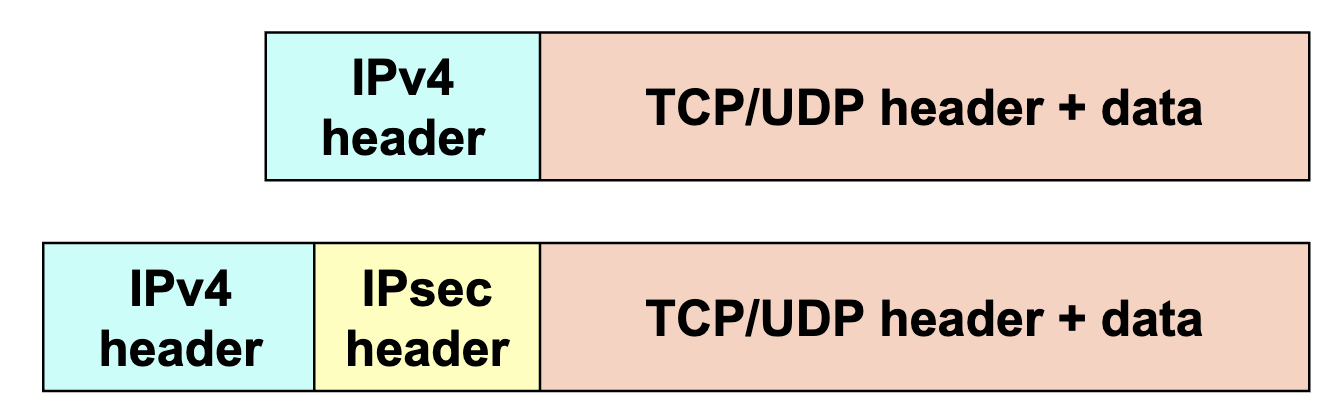
\includegraphics[width=\linewidth]{Images/NetSec/ipsec_transport_mode.png}
    \caption{IPsec transport mode.}
\end{figure}
\end{multicols}

Used for end-to-end security, typically applied by hosts rather than gateways. An exception occurs when the gateway itself requires protection for its own traffic, such as in cases of SNMP or ICMP communication.

\subsection*{IPsec Tunnel Mode}
\begin{center}
    Full encapsulation, computationally heavy.
\end{center}

\begin{multicols}{2}
\raggedcolumns
    Encapsulate the COMPLETE original IP packet within a new IP packet.

    Used to create a VPN (usually by gateway)
\columnbreak

    
\begin{figure}[H]
    \centering
    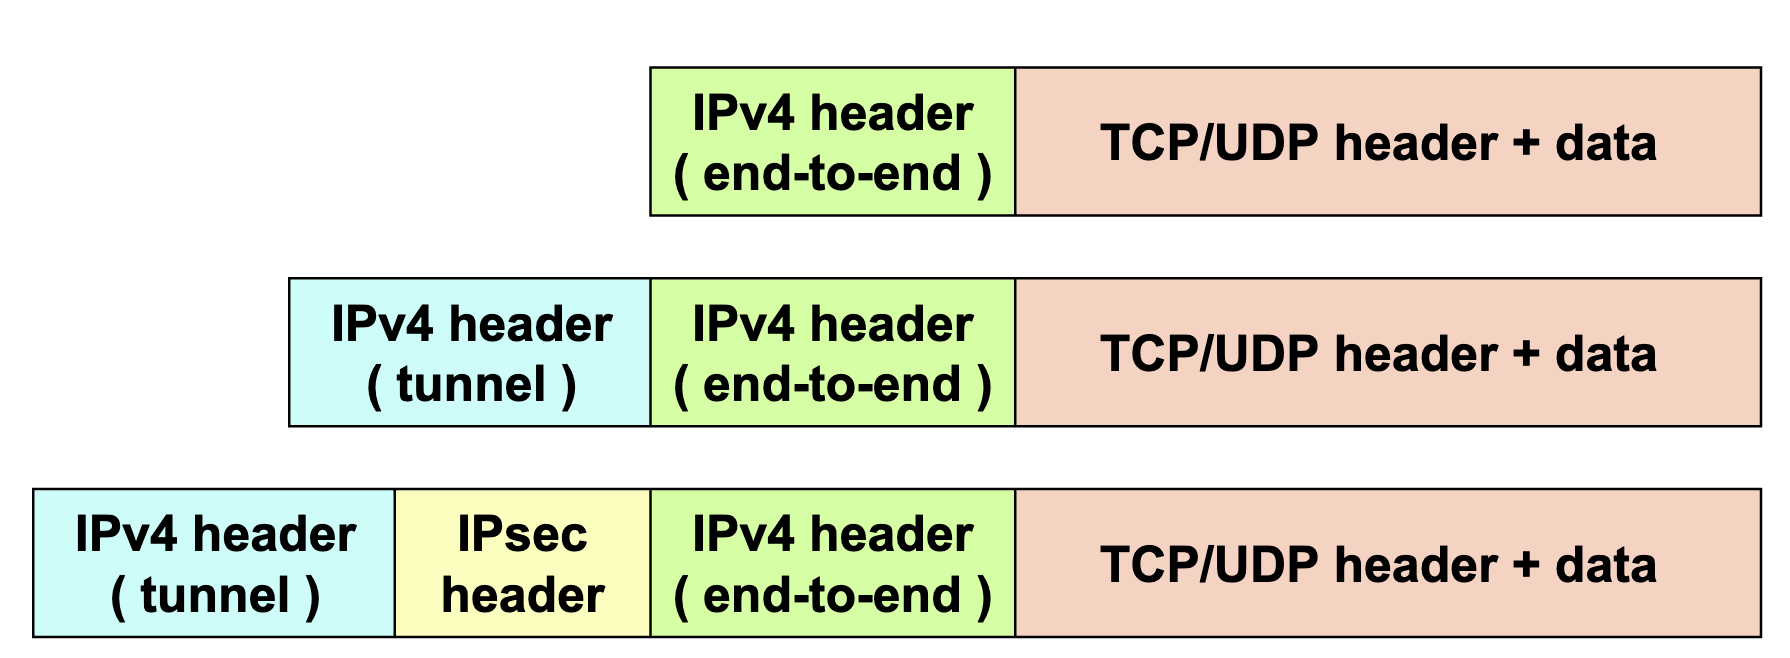
\includegraphics[width=\linewidth]{Images/NetSec/ipsec_tunnel_mode.png}
    \caption{IPsec tunnel mode.}
\end{figure}

\end{multicols}
\subsection{IPsec AH}
\begin{center}
    (Authentication Header - second version RFC-2402)
\end{center}
\textbf{Main points}:
\begin{itemize}
    \item Provides:
    \begin{itemize}
        \item Data integrity and sender authentication for the entire IP packet (MAC computation through keyed-digest), ensuring that the data has not been tampered with and confirming the identity of the sender.
    \end{itemize}
\end{itemize}


\clearpage

\begin{multicols}{2}
    \raggedcolumns
    \textbf{AH v1}, Key features:

    \begin{itemize}
        \item Data integrity and sender authentication for IP packets
        \item Compulsory support of keyed-MD5 (RFC-1828).
        \item Optional support of keyed-SHA-1 (RFC-2402).
    \end{itemize}

\columnbreak

\textbf{AH v2}, Key features:

\begin{itemize}
    \item Data integrity and sender authentication for IP packets.
    \item \textcolor{red}{New!} Partial protection against replay attacks (sequence number).
    \item Support for HMAC-MD5-96 and HMAC-SHA-1/96\footnote{HMAC-SHA1-96 is a variant of the HMAC (Hashed Message Authentication Code) construction that uses the SHA-1 hash function, but with a specific output length of 96 bits (12 bytes), instead of the full 160-bit (20-byte) output of SHA-1.}.
    \begin{itemize}
        \item \textcolor{red}{Be aware! }The output is truncated to 96 bits, though MD5 produces 128 bits and SHA-1 produces 160 bits.
        \item Packets have the same size.
    \end{itemize} 
\end{itemize}
\end{multicols}








\begin{multicols}{2}
\raggedcolumns
    
\begin{tcolorbox}[colback=blue!10!white, colframe=blue!50!white, title=Insight]
    The Security Parameters Index (SPI) is the entry for the Security Association Database (SAD). In the figure rows are 32 bits long.
    \end{tcolorbox}
\columnbreak

    
\begin{figure}[H]
    \centering
    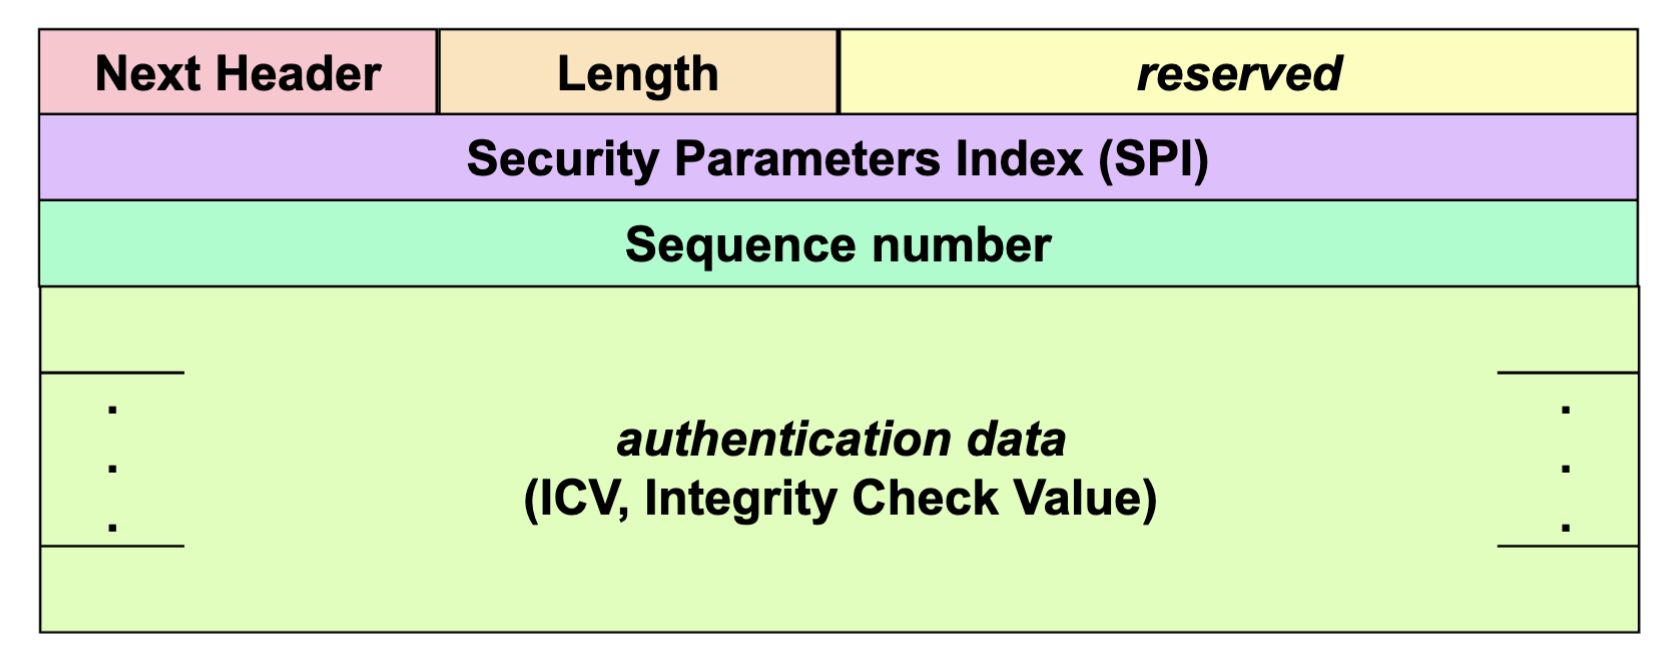
\includegraphics[width=\linewidth]{Images/NetSec/AH_format.png}
    \caption{Authentication Header (AH) format.}
\end{figure}
\end{multicols}

\begin{tcolorbox}[colback=blue!10!white, colframe=blue!50!white, title={For Any Truncated MAC}]
    \begin{itemize}
        \item \textbf{(Pro)}: Less information for the attacker.
        \item \textbf{(Disadvantage)}: Fewer bits to predict for the attacker (reduced search-space).
        \item \textbf{(Do)}: Never truncate to less than half of the hash size $digest\_len\over 2$ (to mitigate the birthday attack length).
        \item \textbf{(Do)}: Never truncate to less than 80 bits (too short for secure use).
    \end{itemize}
\end{tcolorbox}




\clearpage
\subsection{IPsec Packet Receiving}
Need to verify:
\begin{itemize}
    \item \textbf{Authentication}: Ensuring the packet comes from an authentic sender.
    \item \textbf{Integrity}: Ensuring the packet has not been tampered with during transmission.
\end{itemize}

\begin{multicols}{2}
    \raggedcolumns
From the Left Side of the figure:
    \begin{itemize}
        \item The Authentication Header (AH) is extracted to define the Security Parameters Index (SPI), which is used to identify the Security Association (SA) tied to this packet. Simultaneously, the \textbf{Integrity Check Value (ICV)} (keyed-digest) is extracted.
        \item The SPI points to the Security Association (SA) stored in the SAD (Security Association Database), which contains the algorithm, parameters, and keys (exchanged during the key negotiation phase, e.g. using IKE protocol) required also for the MAC computation.
    \end{itemize}


\columnbreak
From the Right Side of the figure:

    \begin{itemize}
        \item The packet undergoes normalization to standardize its format. Normalization resolves any ambiguities in the packet format.
        \item The system computes a Computed Authentication Value (CAV - simply a MAC), for the normalized IP packet using the algorithm and keys from the SA:
    \[
    \text{CAV} = \text{H(Norm\_packet, Key)}
    \]
    Remember that only the leftmost 96 bits are used for comparison.
    \end{itemize}
\end{multicols}

Then the system compares the \textbf{Computed Authentication Value (CAV)} with the \textbf{Received Authentication Value (RAV)}:
\begin{itemize}
    \item If the values \textbf{match}: The packet is from an \textbf{authentic sender} and has \textbf{integrity} \textrightarrow \textcolor{Green}{Packet accepted}.
    \item If the values \textbf{do not match}: The packet is from a \textbf{fake sender and/or has been manipulated} \textrightarrow \textcolor{Red}{Packet rejected}.
\end{itemize}


\begin{figure}[H]
    \centering
  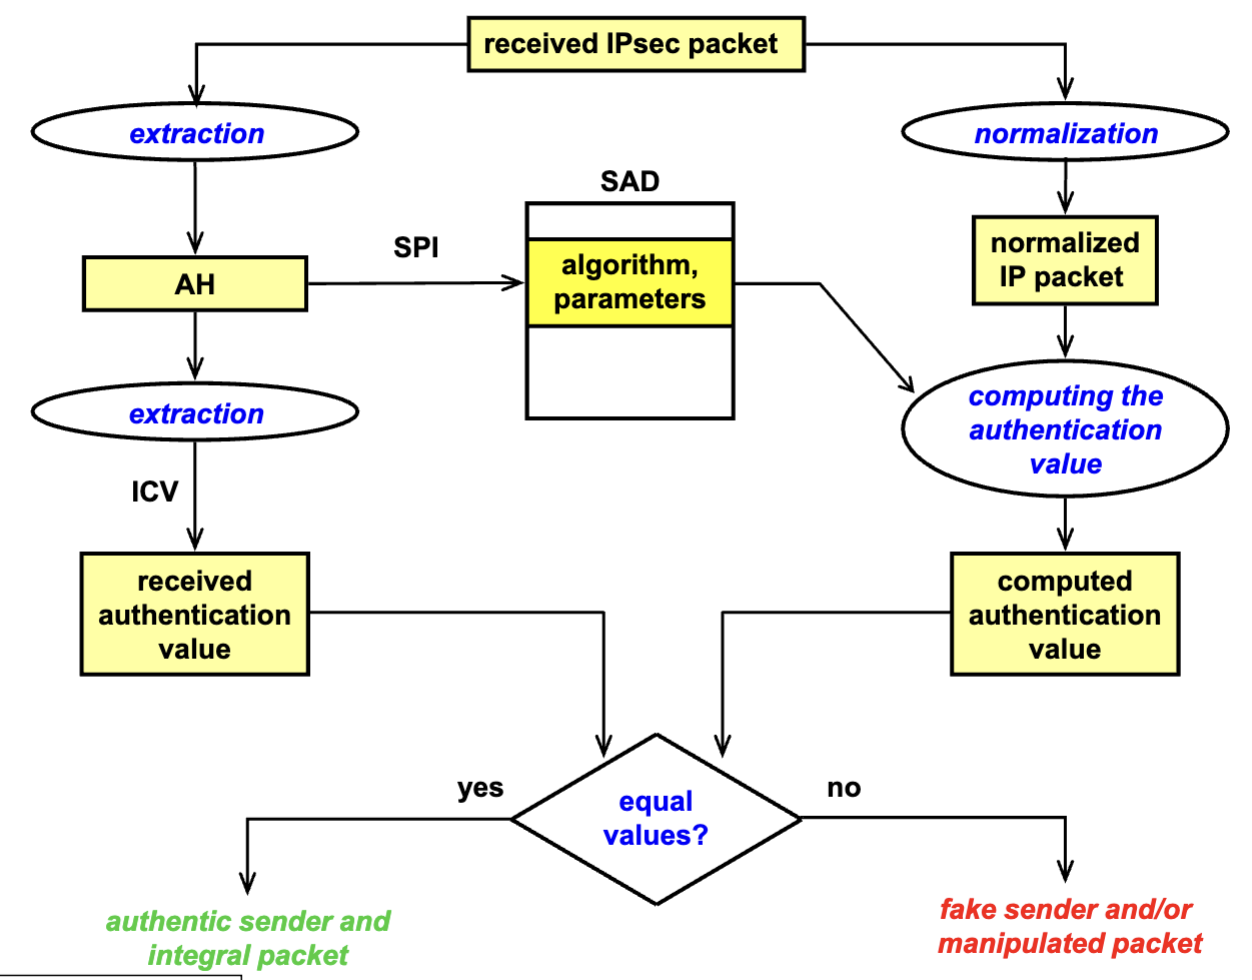
\includegraphics[width=0.5\linewidth]{Images/NetSec/packet_receiving.png}
  \caption{IPsec packet receiving.}
  \label{fig:ipsec_packet_rec}
\end{figure}


\subsection{IPsec ESP}
\begin{center}
    (Encapsulating Security Payload)

    Operates only on the payload for confidentiality.
\end{center}
Like AH, can be applied after the modes. Base mechanism: \textbf{DES-CBC} (RFC-1829), but other mechanisms are also possible.

\begin{multicols}{2}
    \raggedcolumns
    \textbf{ESP v1} (RFC-1827):

    Gave only \textbf{confidentiality} to the payload.

\columnbreak

\textbf{ESP v2} (RFC-2406):

Provides confidentiality and also offers \textbf{authentication} but only for the IP payload, not the header.
\end{multicols}


\begin{center}
    \textbf{ESP in Transport Mode}
\end{center}


\begin{multicols}{2}
    \raggedcolumns
    \begin{itemize}
        \item \textbf{Advantages}: The payload is hidden.
        \item \textbf{Downsides}: The header remains in clear
    \end{itemize}

\columnbreak

\begin{figure}[H]
    \centering
  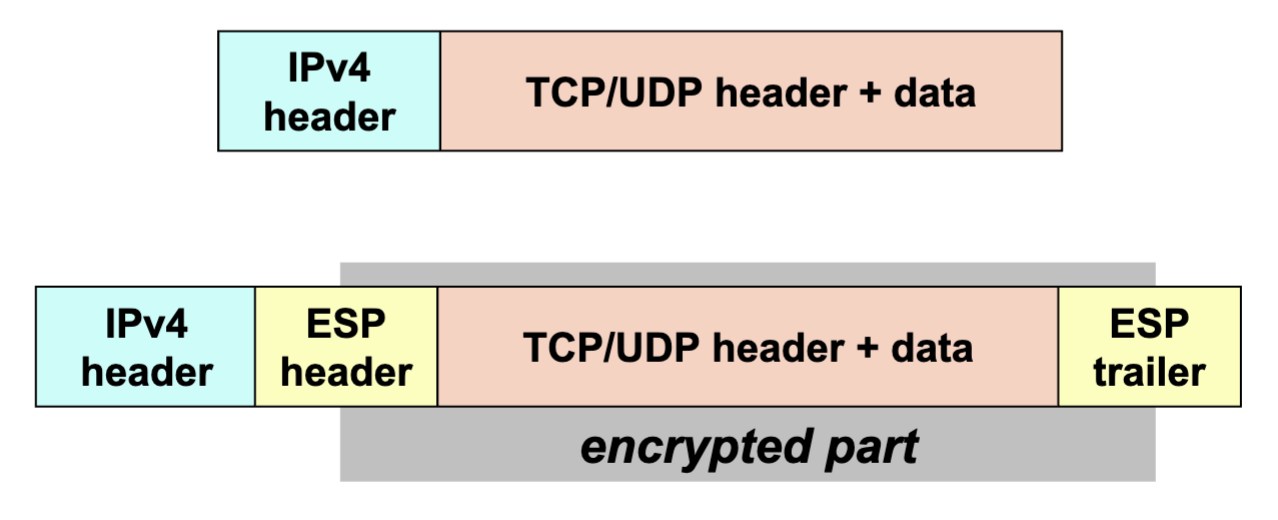
\includegraphics[width=\linewidth]{Images/NetSec/esp_transport_mode.png}
  \caption{ESP in transport mode.}
\end{figure}
\end{multicols}

\begin{tcolorbox}[colback=red!10!white, colframe=red!70!black, coltitle=white, title=Bad News for Network Management]
    The fact that ESP in transport mode encrypts the packet's payload can pose issues for network management, particularly in areas such as traffic monitoring, QoS (Quality of Service), filtering, and intrusion detection.
\end{tcolorbox}



\begin{center}
    \textbf{ESP in Tunnel Mode}
\end{center}


\begin{multicols}{2}
    \raggedcolumns
    \begin{itemize}
        \item \textbf{Advantages}: Hides both the payload and (original) header (\textcolor{red}{same problems for network management as ESP in transport mode}).
        \item \textbf{Downsides}: Larger packet size.
    \end{itemize}

\columnbreak

\begin{figure}[H]
    \centering
    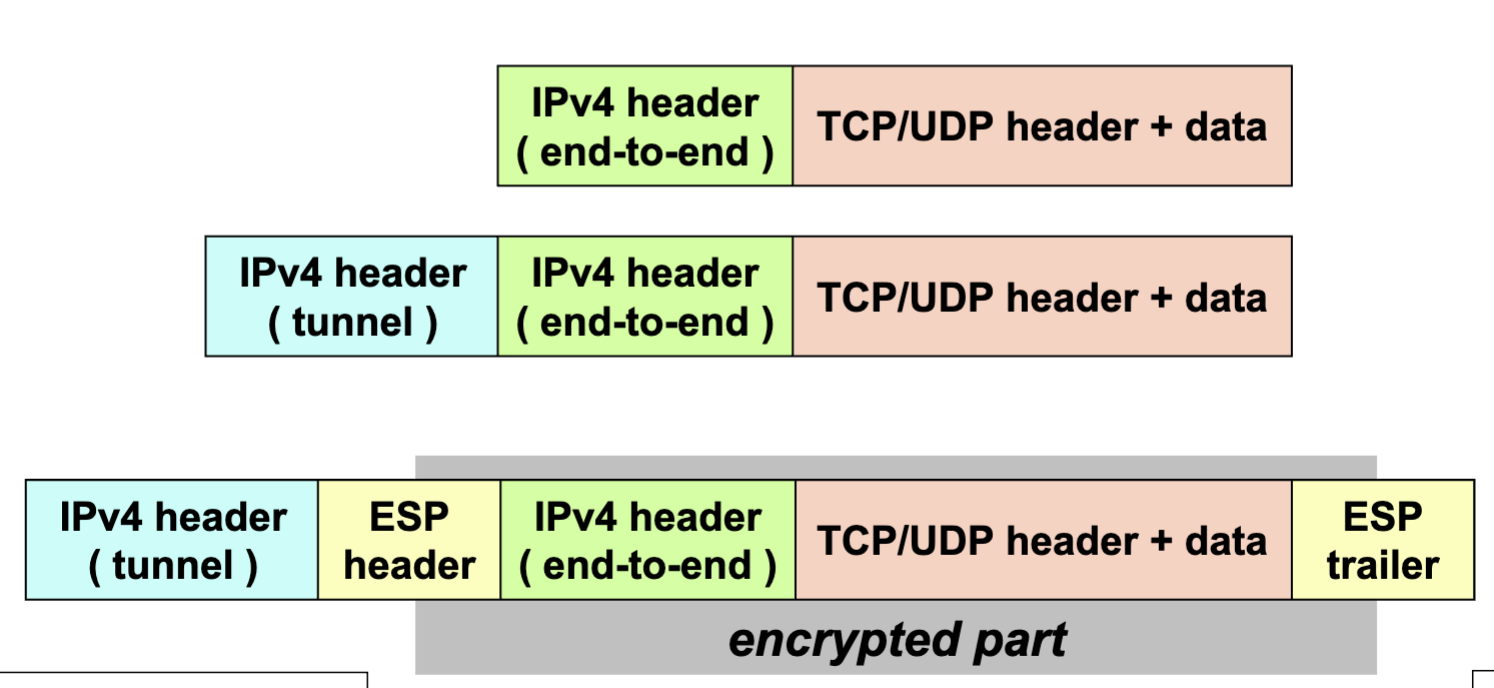
\includegraphics[width=\linewidth]{Images/NetSec/esp_tunnel_mode.png}
    \caption{ESP in tunnel mode.}
\end{figure}
\end{multicols}

\begin{tcolorbox}[colback=red!10!white, colframe=red!70!black, coltitle=white, title=Be aware]
    In ESP tunnel mode, the entire original IP packet (including both the header and the payload) is encapsulated within a new IP packet. This means that the \textbf{intermediate network devices (e.g., routers, switches) can only see the border router} (the one initiating or terminating the tunnel) and not the internal nodes generating the packets.
\end{tcolorbox}



\subsection*{IPsec Implementation Details}
Key features:
\begin{itemize}
    \item \textbf{UI crypto-suites} (RFC-4308) for interoperability
    \item \textbf{VPN-}(type)\textbf{A} = \texttt{ESP/3DES-CBC/HMAC-SHA1-96}
    \item \textbf{VPN-B} = \texttt{ESP/AES-128-CBC/AES-XCBC-MAC-96}
    \item \textbf{NULL algorithms for ESP}:
    \begin{itemize}
        \item Used for \textbf{authentication} or \textbf{privacy}, but \textbf{not simultaneously}
        \item Trade-off between \textbf{protection} (no header confidentiality) and \textbf{performance}
    \end{itemize}
    \item \textbf{Sequence number}:
    \begin{itemize}
        \item Provides \textbf{partial protection} from replay attacks
        \item Minimum window size of \textbf{32 packets} (64 packets recommended)
        \item Creation is mandatory for the sender, but verification is optional for the receiver (this is announced during \textbf{SA negotiation}). \textcolor{red}{the receiver can be replayed if possible!}
    \end{itemize}
    \item \textbf{VPN concentrator}: A special-purpose appliance that acts as the terminator of an IPsec tunnel:
    \begin{itemize}
        \item Used for remote access by individual clients.
        \item Facilitates the creation of site-to-site VPNs.
        \item Offers very high performance relative to its low cost.
    \end{itemize}
\end{itemize}



\subsection{IPsec Replay Protection}
\begin{center}
    (Due to the best-effort nature of the IP protocol)
\end{center}

\begin{multicols}{2}
\raggedcolumns
    Main points:
    \begin{itemize}
        \item At SA creation, the sender initializes the sequence number to 0.
        \item When sending a packet, the sender increments the sequence number.
        \item When the sequence number reaches \( 2^{32} - 1 \) (i.e., \( 4.29 \cdot 10^{9}\)), a new Security Association (SA) should be negotiated.
    \end{itemize}
\columnbreak

    
\begin{figure}[H]
    \centering
  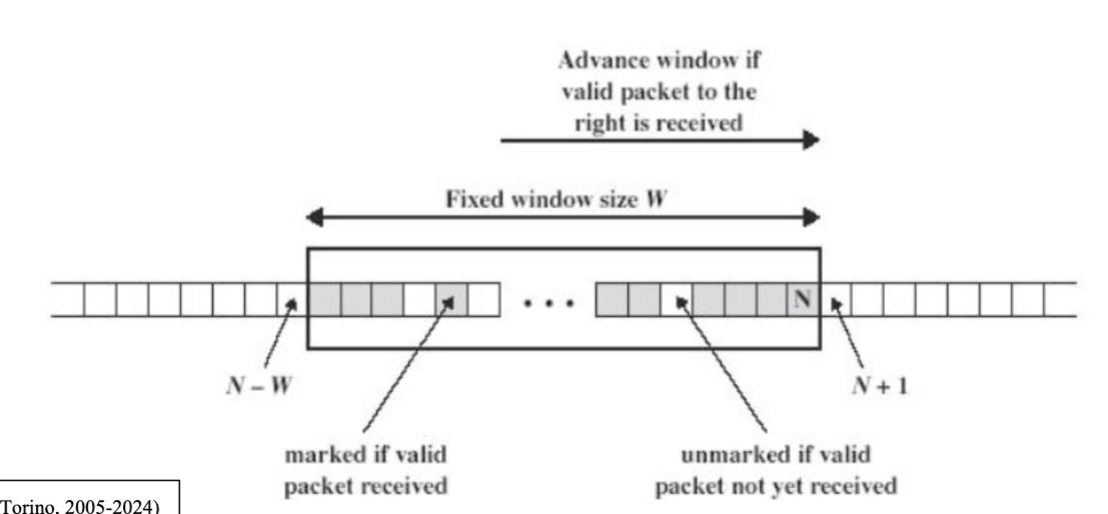
\includegraphics[width=\linewidth]{Images/NetSec/ipsec_replay_protection.png}
  \caption{IPsec moving window or replay protection.}
\end{figure}
\end{multicols}

\textbf{Moving window}:
        \begin{itemize}
            \item \textbf{Outside the window}, there is no replay protection. You must choose between security (implicitly negating incoming packets) or performance (implicitly accepting incoming packets).
            \item \textbf{Inside the window}, replay protection is enforced.
        \end{itemize}


\subsection{IPsec v3}
Key features:
\begin{itemize}
    \item \textbf{AH} is optional, \textbf{ESP} is mandatory.
    \item Support for single-source multicast\footnote{In this communication model, only one source node sends the multicast data, and the data is distributed to multiple receivers that have expressed interest in receiving the multicast stream.}.
    \item \textbf{ESN} (Extended Sequence Number):
    \begin{itemize}
        \item 64 bits (but only the 32 least significant bits are transmitted).
        \item Default when using \textbf{IKEv2}, but its usage must be explicitly negotiated.
        \item \textcolor{red}{Prevention of Sequence Number Wraparound (traffic disruption)}
    \end{itemize}
    \item Support for authenticated encryption (\textbf{AEAD}).
    \item Clarifications about \textbf{SA} (Security Association) and \textbf{SPI} (Security Parameter Index) for faster lookup.
\end{itemize}

\subsubsection*{Algorithms}
\begin{center}
    (RFC-4305)
\end{center}

\begin{itemize}
    \item \textbf{For integrity and authentication:}
    \begin{itemize}
        \item (MAY) HMAC-MD5-96
        \item (MUST) HMAC-SHA-1-96
        \item (SHOULD, recommended) AES-XCBC-MAC-96
        \item (MUST) NULL (only for ESP)
    \end{itemize}
    \item \textbf{For privacy:}
    \begin{itemize}
        \item (MUST) NULL
        \item (MUST NOT) 3DES-CBC
        \item (SHOULD, recommended) AES-128-CBC
        \item (SHOULD) AES-CTR
        \item (SHOULD NOT) DES-CBC
    \end{itemize}
    \item \textbf{For authenticated encryption (AEAD mode):}
    \begin{itemize}
        \item AES-CCM
        \item AES-CMAC
        \item ChaCha20 with Poly1305
    \end{itemize}
    \item \textbf{For authentication and integrity:}
    \begin{itemize}
        \item HMAC-SHA-256-128
        \item HMAC-SHA-384-192
        \item HMAC-SHA-512-256
    \end{itemize}

\end{itemize}

\subsection{IPsec Traffic Flow Confidentiality}
\begin{center}
    Strategy of obscuring traffic patterns in a network.
\end{center}
Is a concept in IPsec designed to obscure traffic patterns in a network, making it difficult for attackers or eavesdroppers to infer information based on the size or timing of network traffic.

Key features:
\begin{itemize}
    \item Padding in ESP:
    \begin{itemize}
        \item Placed after the payload and before the normal padding.
        \item The receiver must be able to compute the original size of the payload (e.g., possible with IP, UDP, and ICMP payloads).
    \end{itemize}
    \item Support for "dummy packets".
        \begin{itemize}
            \item Packets that contain no meaningful data and are primarily used for traffic flow obfuscation rather than actual communication.
            \item \texttt{Next\_Header}=59: Value in the IP AH header that is used to indicate that the packet is a dummy (with no real data).
            \item The use of dummy packets is \textcolor{red}{meaningful only in encrypted traffic}. If the traffic is not encrypted, attackers can easily analyze the packets and distinguish between real data and dummy packets based on their content.
        \end{itemize}
\end{itemize}

\begin{tcolorbox}[colback=blue!10!white, colframe=blue!50!white, title=Cool Information]
    The mere fact that a communication is established provides valuable information to eavesdroppers.
\end{tcolorbox}

\begin{tcolorbox}[colback=red!10!white, colframe=red!70!black, coltitle=white, title=Beware]
        There will always be a \textbf{loss of performance} when using this concept.
\end{tcolorbox}

\clearpage
\subsection{IPsec Implementations}

\subsubsection{IPsec for End-to-End Security}

\begin{center}
    Transport-Mode, host-to-host.
\end{center}

The diagram \ref{fig:EESec} illustrates the use of IPsec in transport mode to establish a secure virtual channel between two individual hosts over a wider network (WAN).



\begin{multicols}{2}
\raggedcolumns
    Main points:
    \begin{itemize}
        \item LAN traffic is protected.
        \begin{itemize}
            \item Each host encapsulates its data (not the variable fields of the header) before transmission.
        \end{itemize}
        \item High computational effort: each device must implement IPsec.
        \item The gateways act as border elements and do not process IPsec packets.
    \end{itemize}
\columnbreak

\begin{figure}[H]
    \centering
  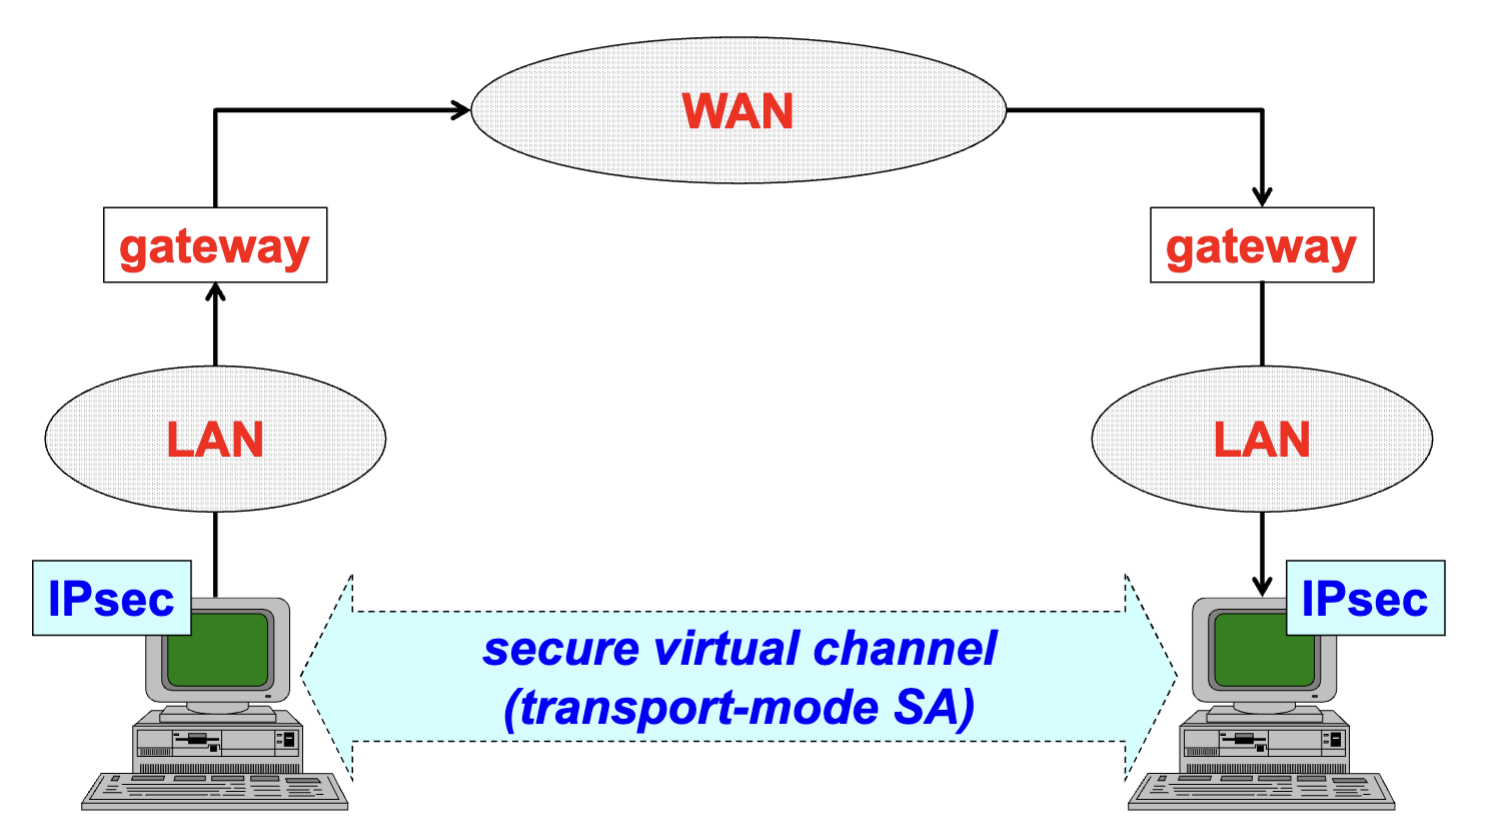
\includegraphics[width=\linewidth]{Images/NetSec/end_to_end_security.png}
  \caption{End-to-End security implementation.}
  \label{fig:EESec}
\end{figure}
\end{multicols}

\subsubsection{IPsec for Basic VPN}
\begin{center}
    Tunnel-Mode, gateway-to-gateway.
\end{center}
The diagram \ref{fig:basicVPN} illustrates the use of IPsec in tunnel mode to establish a secure virtual channel between two networks over a wider network (WAN).

\begin{multicols}{2}
\raggedcolumns
    Main points:
    \begin{itemize}
        \item LAN traffic is \textcolor{red}{not} protected.
        \item IPsec is implemented on the company's gateways.
        \item The IP packets in the external network are fully encapsulated (tunnel mode).
    \end{itemize}
\columnbreak

\begin{figure}[H]
    \centering
  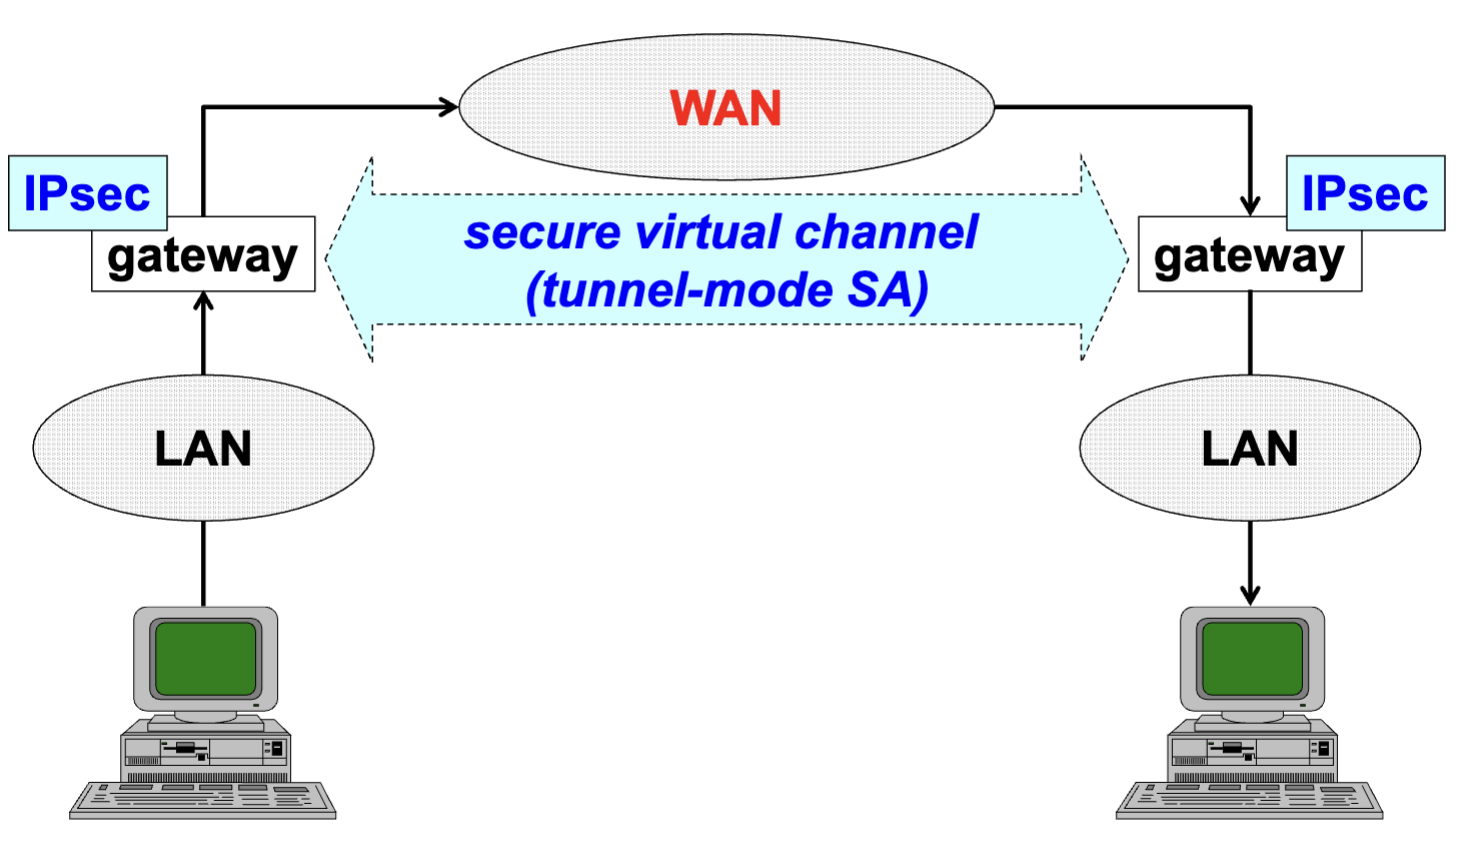
\includegraphics[width=\linewidth]{Images/NetSec/basic_vpn.png}
  \caption{Basic VPN implementation.}
  \label{fig:basicVPN}
\end{figure}
\end{multicols}

\clearpage

\subsubsection{IPsec for End-to-End Security with Basic VPN}

\begin{multicols}{2}
\raggedcolumns

    Main points:
    \begin{itemize}
        \item LAN traffic is \textcolor{red}{not} protected within the local network (transport mode).
        \item External LAN traffic is fully protected, ensured by tunnel mode.
        \item IPsec is implemented on the company's gateways and hosts.
        \end{itemize}
\columnbreak

\begin{figure}[H]
    \centering
    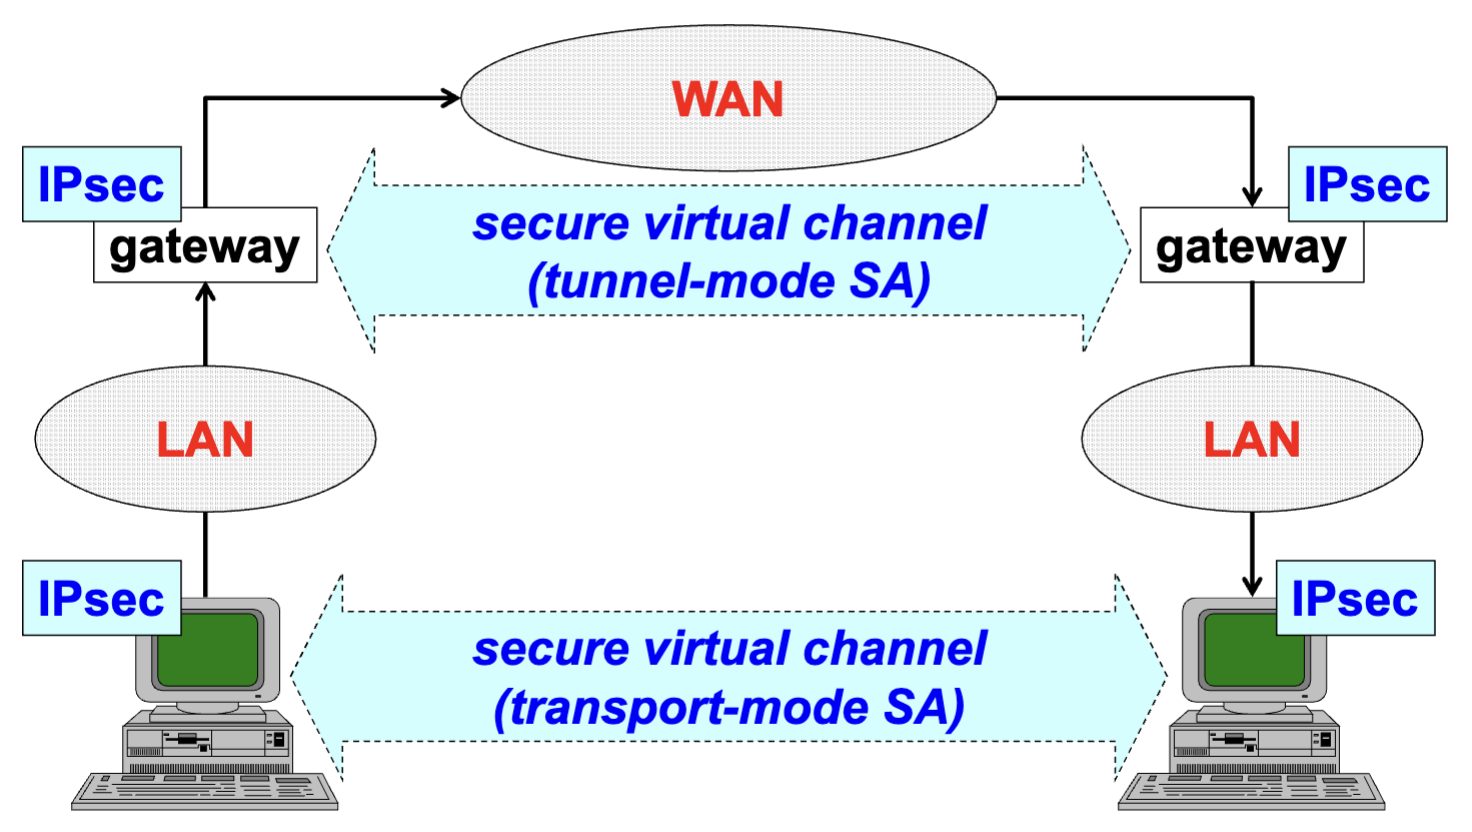
\includegraphics[width=\linewidth]{Images/NetSec/end_vpn.png}
    \caption{End-to-End Security with basic VPN implementation.}
    \label{fig:end_vpn}
\end{figure}
\end{multicols}

\subsubsection{IPsec for Secure Gateway}
\begin{center}
    Tunnel mode, host-to-gateway.
\end{center}

\begin{multicols}{2}
\raggedcolumns
    Main points:
    \begin{itemize}
        \item The devices securely communicate with the gateway over an external network.
    \end{itemize}
\columnbreak

\begin{figure}[H]
    \centering
  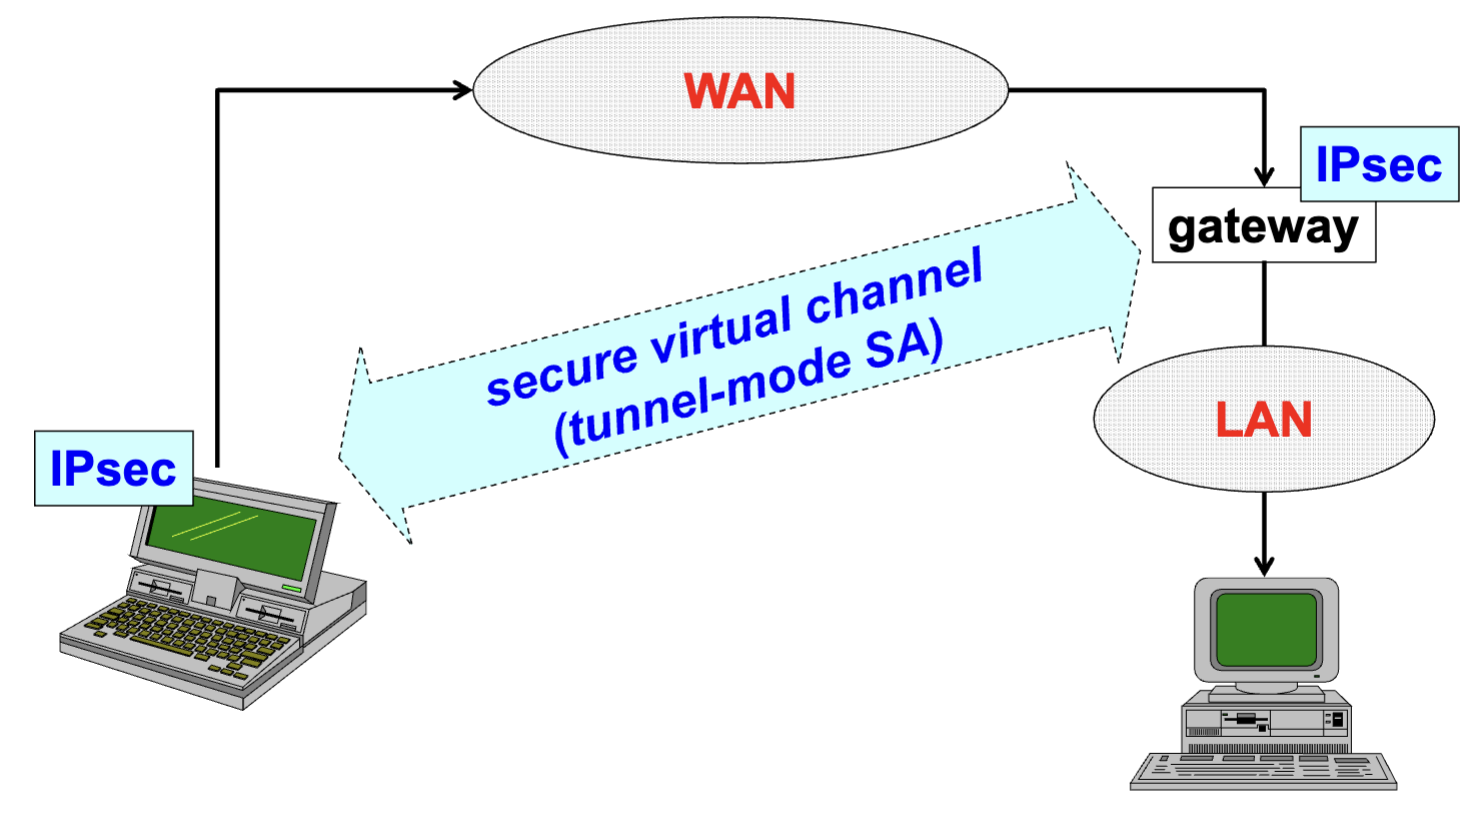
\includegraphics[width=\linewidth]{Images/NetSec/secure_gateway.png}
  \caption{Secure gateway implementation.}
  \label{fig:secgat}
\end{figure}

\end{multicols}

\subsubsection{IPsec for Secure Remote Access}
\begin{center}
    Transport mode, host-to-gateway + Tunnel mode, gateway-to-gateway.
\end{center}

The figure \ref{fig:gat_end} depicts an end-to-end security layered on top of secure gateway architecture. 



\begin{multicols}{2}
\raggedcolumns
    Key features:
    \begin{itemize}
        \item \textcolor{red}{Problem: }\textbf{Key Management}: Keys or certificates must be exchanged between the communicating endpoints, bypassing the gateway's control.
    \end{itemize}
\columnbreak

\begin{figure}[H]
    \centering
  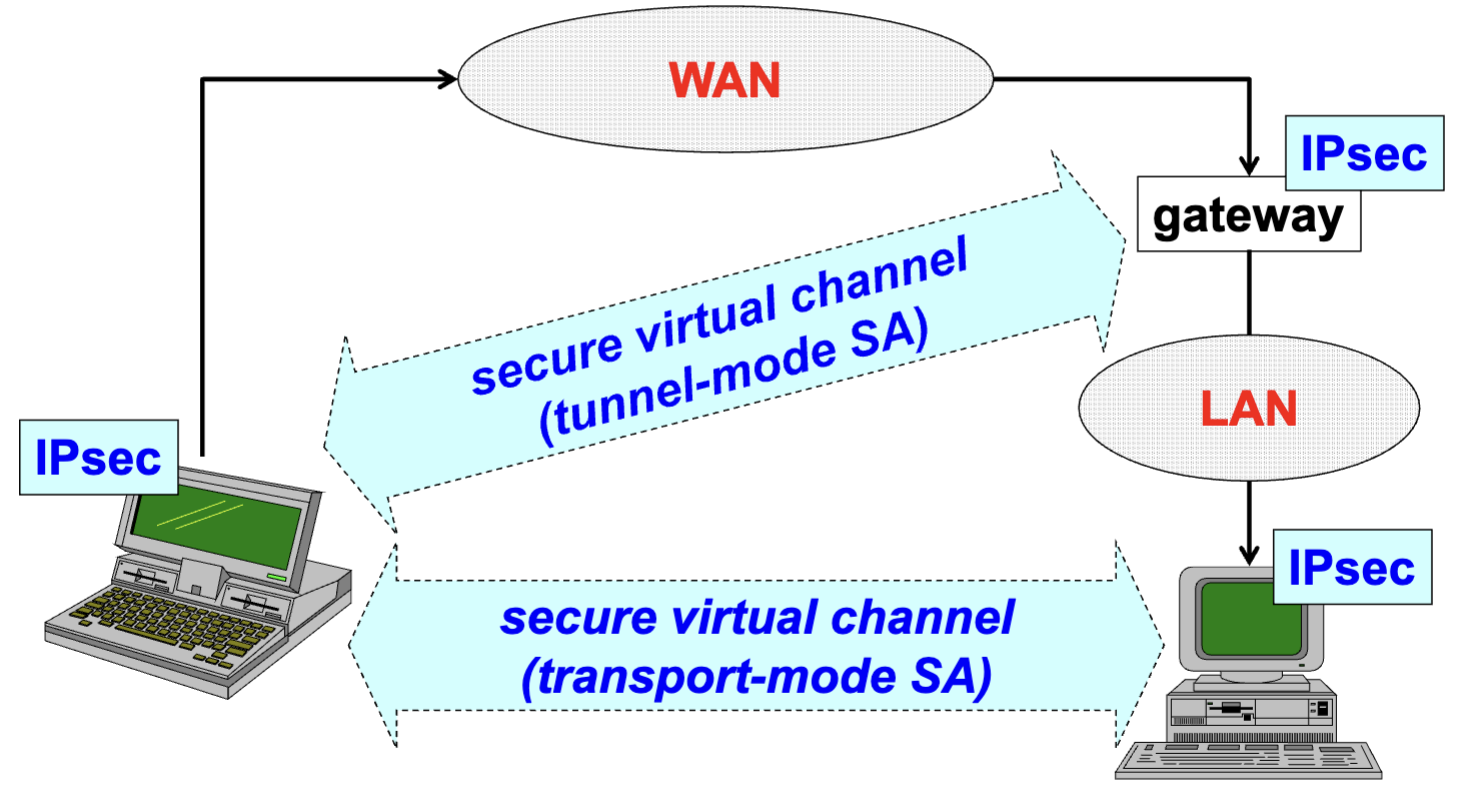
\includegraphics[width=\linewidth]{Images/NetSec/gatsec_end.png}
  \caption{Gateway-based security with end-to-end security.}
  \label{fig:gat_end}
\end{figure}
\end{multicols}


\clearpage

\subsubsection{IPsec for Anonymous Navigation}
\begin{center}
    Tunnel mode, VPN-server. Typical implementation of VPN.
\end{center}
The figure \ref{fig:anonnav} illustrates a scenario of anonymous navigation using a VPN (Virtual Private Network) setup.

The packet is fully encapsulated (tunnel mode) and sent to the VPN server, but full protection over the packet is not guaranteed.



\begin{multicols}{2}
    \raggedcolumns


    \begin{itemize}
        \item The VPN server:
        \begin{itemize}
            \item Is a trusted intermediary that establishes a secure communication channel with the client. 
        \end{itemize}
        \item Secure Virtual Channel (tunnel-mode):
    \end{itemize}
\columnbreak

    
\begin{figure}[H]
    \centering
  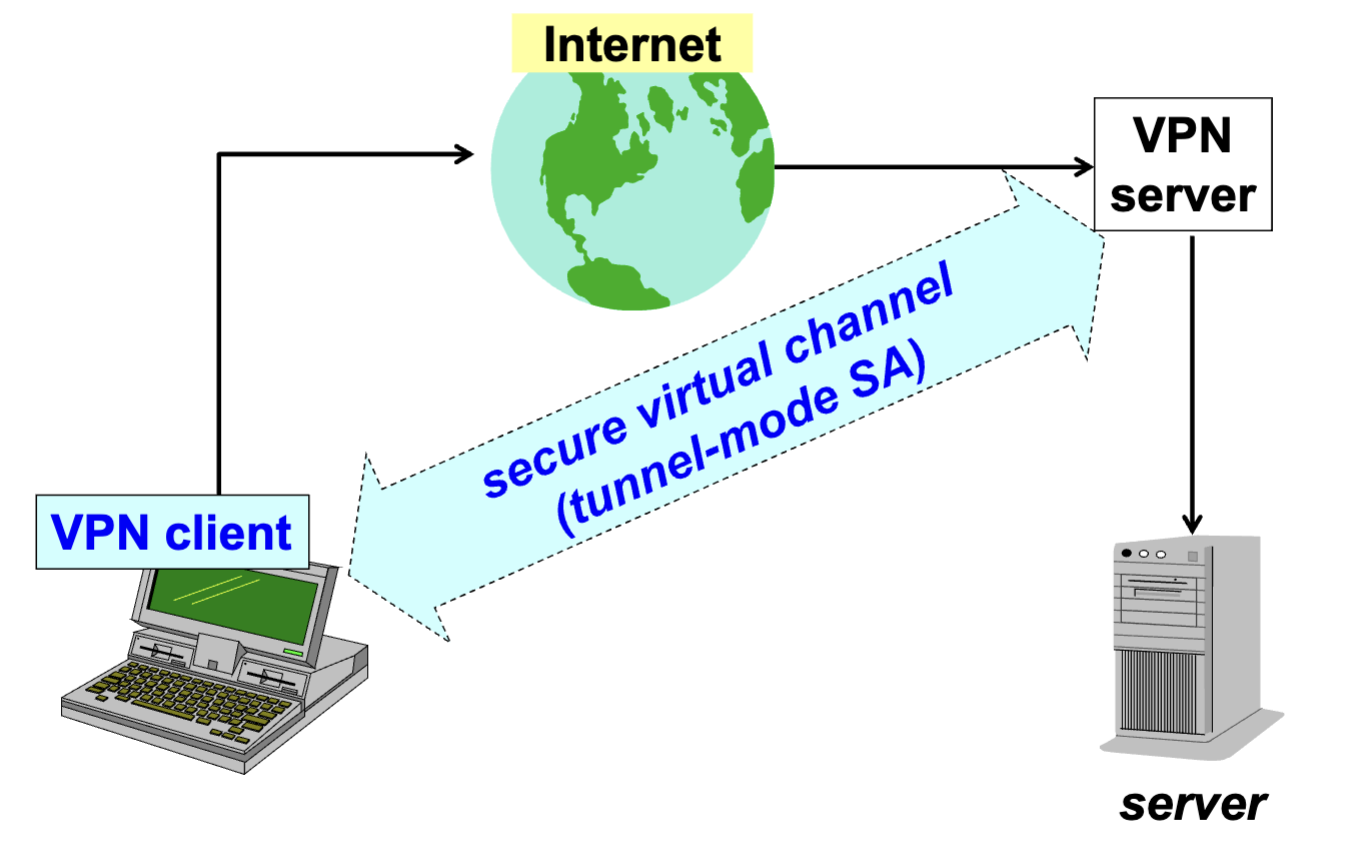
\includegraphics[width=\linewidth]{Images/NetSec/anonnav.png}
  \caption{Anonymous navigation.}
  \label{fig:anonnav}
\end{figure}

\end{multicols}

\subsection{IPsec Key Management}
The key management is a very important component of IPsec. Provides to the IPsec parties the symmetric keys used for packet authentication/integrity and/or encryption.

Key distribution:
\begin{itemize}
    \item OOB (Out-Of-Band, e.g. manual, installing pre-shared key).
    \item Automatic in-band (e.g. IKE): The keys are exchanged during the negotiation of the IPsec SAs.
\end{itemize}

\subsubsection{Internet Security Association and Key Management Protocol}
\begin{center}
    (ISAKMP - RFC-2408)
\end{center}

Key features:
\begin{itemize}
    \item Provides a framework for establishing, managing, and deleting Security Associations (SAs).
    \item Does not dictate a specific key exchange method but allows for flexibility by integrating different protocols (e.g., OAKLEY).
    \item Reuse of ISAKMP SA: The same ISAKMP SA can be reused for negotiating\footnote{SA Negotiation: Handles the negotiation of SA parameters required for IPsec traffic, such as encryption algorithms and key lifetimes.} multiple IPsec SAs, optimizing performance.
\end{itemize}
\subsubsection{OAKLEY}
\begin{itemize}
    \item A protocol for authenticated key (symmetric) exchanges between parties.
    \item \underline{Only} used for automatic in-band key distribution.
\end{itemize}

\subsubsection{Internet Key Exchange}
\begin{center}
    (IKE - RFC-2409 IKEv1 - RFC-7296 IKEv2)

    Automatic in-band key exchange protocol.
\end{center}
\[
ISAKMP + OAKLEY
\]

Used for the secure negotiation of IPsec SAs, including the exchange of keys and authentication. Combines the functionalities of ISAKMP and OAKLEY into a single protocol.

Purpose:
\begin{itemize}
\item \textbf{Creation of ISAKMP SA}: The first step is to establish a secure channel (called the ISAKMP SA) to protect subsequent negotiations. This channel is itself negotiated and secured by IKE.
\item \textbf{Negotiation of IPsec SAs}: After the ISAKMP SA is established, it is used to negotiate the IPsec SAs, which define the parameters for securing IPsec-protected traffic.
\end{itemize}

\hfill

\textbf{IKE - Operations}

\vspace{0.2cm}

Purpose of Phase 1:

\begin{center}
    Negotiates a bidirectional ISAKMP (Internet Security Association and Key Management Protocol) Security Association (SA), which establishes a secure, encrypted channel for further communication.
\end{center}
Purpose of Phase 2:
\begin{center}
    Negotiates the IPsec Security Association (SA), which defines how the traffic will be encrypted, authenticated, and tunneled.
\end{center}

\begin{figure}[H]
    \centering
  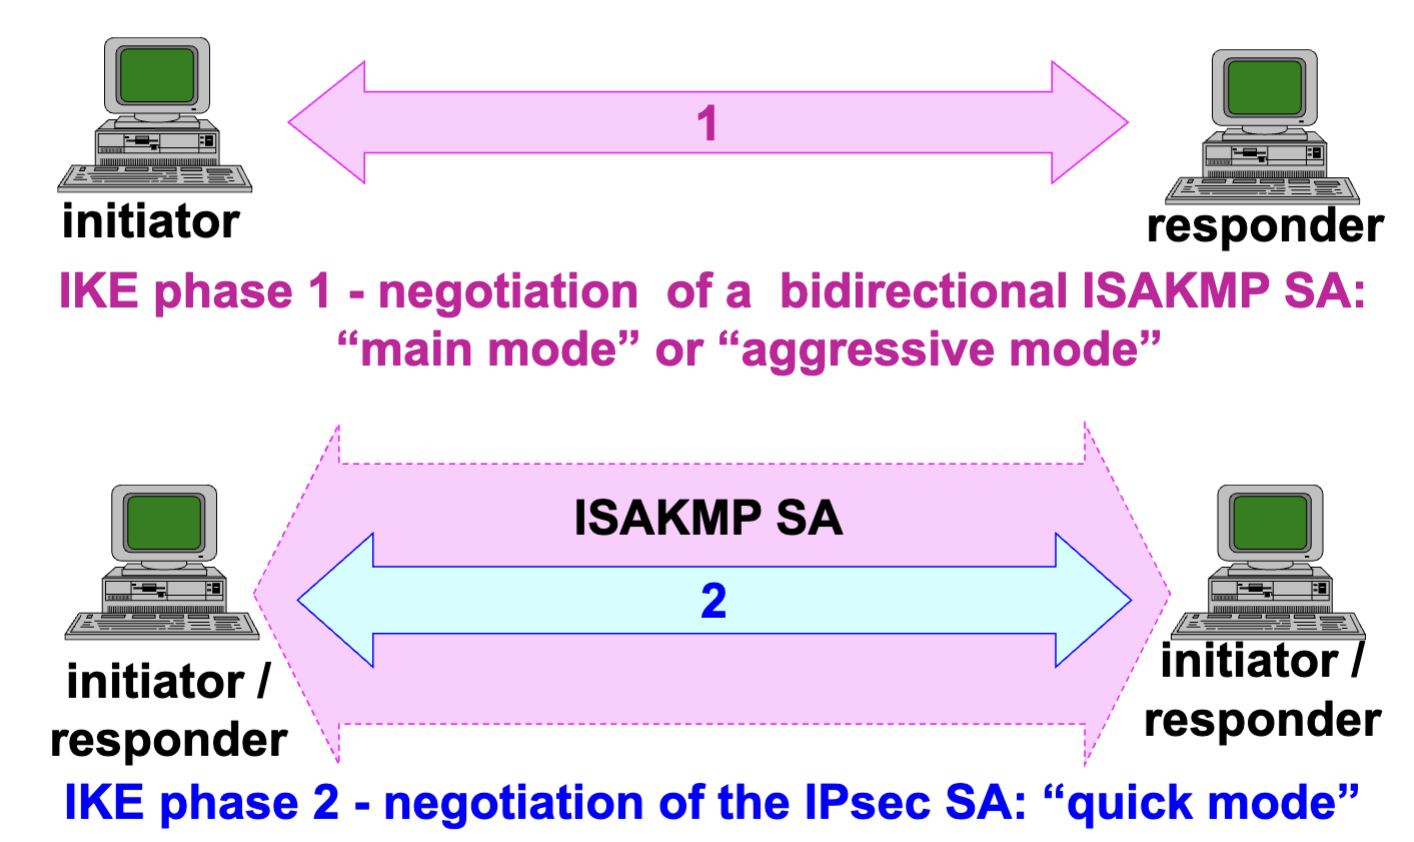
\includegraphics[width=0.5\linewidth]{Images/NetSec/ike_operations.png}
  \caption{IKE operations.}
\end{figure}


\clearpage
\textbf{IKE - Modes of Operation}
\vspace{0.2cm}


\begin{itemize}
    \item \textbf{Main mode}:
    \begin{itemize}
        \item 6 messages exchanged (both sides authenticate each other and agree on key exchange parameters).
        \item \textcolor{red}{Identity Protection}: The parties exchange their identities in a secure form to prevent them from being visible on the network. This protects not only the IP addresses but also any application layer parameters (such as hostnames or other identifiers).
        \item Secure exchange of cryptographic material (e.g., Diffie-Hellman keys) between the initiator and responder.
    \end{itemize}
    \item \textbf{Aggressive mode}: 3 messages, faster than Main Mode but does not protect the parties' identities (such as IP addresses or hostnames). 
    \item \textbf{Quick mode}: 3 messages exchanged, and used for the negotiation of the IPsec Security Association (SA) after the completion of Phase 1. It focuses on securing the data channel and defining IPsec parameters (e.g., encryption and authentication methods).
    \item \textbf{New group mode}: 2 messages, used for renegotiating the Diffie-Hellman group and refreshing key material. The existing SA remains open, but a new key is negotiated after a predefined number of packets (or time).
\end{itemize}

\hfill

\textbf{Authentication Methods}

\hfill

\begin{itemize}
    \item \textbf{Digital signature}: \textcolor{Blue}{non-repudiation} of the IKE negotiation.
    \item \textbf{Public key Encryption}: \textcolor{Blue}{identity protection} in the aggressive mode.
    \item \textbf{Revised Public Key Encryption}: \textcolor{Blue}{identity protection} and less expensive, only 2 public-key operations.
    \item \textbf{Pre-Shared Key}: The party ID is typically the IP address, which can be problematic for mobile users due to the frequent changes in their IP addresses.
\end{itemize}

\subsection{Applicability of IPsec}
Scenarios, conditions, or environments where the IPsec protocol can be used effectively:
\begin{itemize}
    \item Only for unicast packets (no support for broadcast, multicast, or anycast).
    \item Between parties that have activated a Security Association (SA), which can be established:
    \begin{itemize}
        \item Using shared keys.
        \item Using X.509 certificates.
    \end{itemize}
    \item Therefore, IPsec is used in \textbf{"closed" groups} (it cannot be public, but new users can be registered).
\end{itemize}

\clearpage

\section{IP (In)security}
(LOOK AT THE SLIDES FOR MORE INFORMATION)
\begin{itemize}
    \item IP addresses are not authenticated.
    \item Packets are not protected in terms of:
    \begin{itemize}
        \item Integrity.
        \item Authentication.
        \item Confidentiality.
        \item Protection against replay attacks.
    \end{itemize}
    \item As a result, all protocols that use IP as their carrier are vulnerable to attacks, with a particular impact on "service" protocols (i.e., non-application protocols, such as ICMP, IGMP, DNS, RIP, etc.).
\end{itemize}

\section{ICMP Security}
\textbf{Internet Control Message Protocol (ICMP)}: A vital protocol for network management and diagnostics.
\begin{itemize}
    \item Many attacks are possible because ICMP lacks authentication and security measures.
    \item Common ICMP functions:
    \begin{itemize}
        \item Echo request/reply (used for pinging).
        \item Destination unreachable (network, host, protocol, or port unreachable).
        \item Source quench (used to signal congestion).
        \item Redirect (used for routing updates).
        \item Time exceeded (indicates that the datagram has expired in transit).
    \end{itemize}
\end{itemize}

\begin{tcolorbox}[colback=blue!10!white, colframe=blue!50!white, title=ICMP and IPsec]
ICMP is used for global purposes, so IPsec cannot be implemented with it (since IPsec is intended for use in "closed" groups).
\end{tcolorbox}

\section{DNS Security}
\begin{center}
    (Domain Name System)
\end{center}

\begin{itemize}
    \item \textbf{Translation}: 
    \begin{itemize}
        \item From names to IP addresses
        \item From IP addresses to names
    \end{itemize}
    \item Vital service
    \item Queries over port 53/UDP
    \item Zone transfers over port 53/TCP
    \item No built-in security: \textbf{DNSSEC} (DNS Security Extensions) is under development/deployment to provide security features.
\end{itemize}

\subsection*{DNS Architecture}
\begin{center}
    (Architecture of Iterative Query)
\end{center}

In an \textit{iterative query} in the context of DNS (Domain Name System), the client (typically a resolver) queries a DNS server, which either provides an answer or refers the client to another server that may have the answer. The process involves the following steps:

\begin{itemize}
    \item \textbf{Client (Resolver)}: The client initiates the query by contacting a DNS server.
    \item \textbf{DNS Server (Initial Resolver)}: If the server knows the answer (i.e., it has the requested record in its cache or database), it returns the result to the client. If it doesn't know the answer, it provides a \textit{referral} to another DNS server (usually a higher-level server, such as a root DNS server or an authoritative server for a particular domain).
    \item \textbf{Referral Process}: The client then contacts the referred server, which either provides the answer or refers the client further (if necessary). This process repeats until the client either gets the final answer or encounters a server that has authoritative data for the queried domain.
    \item \textbf{No Recursion by Server}: In an iterative query, the DNS server does \textit{not} perform recursion. It only returns what it knows or refers to other servers. The client is responsible for following the chain of referrals.
\end{itemize}

In summary, in iterative querying, the DNS resolver follows the chain of referrals to find the requested information. Each server in the chain only provides the best answer it can (either the requested data or a referral to another server), and the client handles further queries until the answer is found.

\begin{figure}[H]
    \centering
  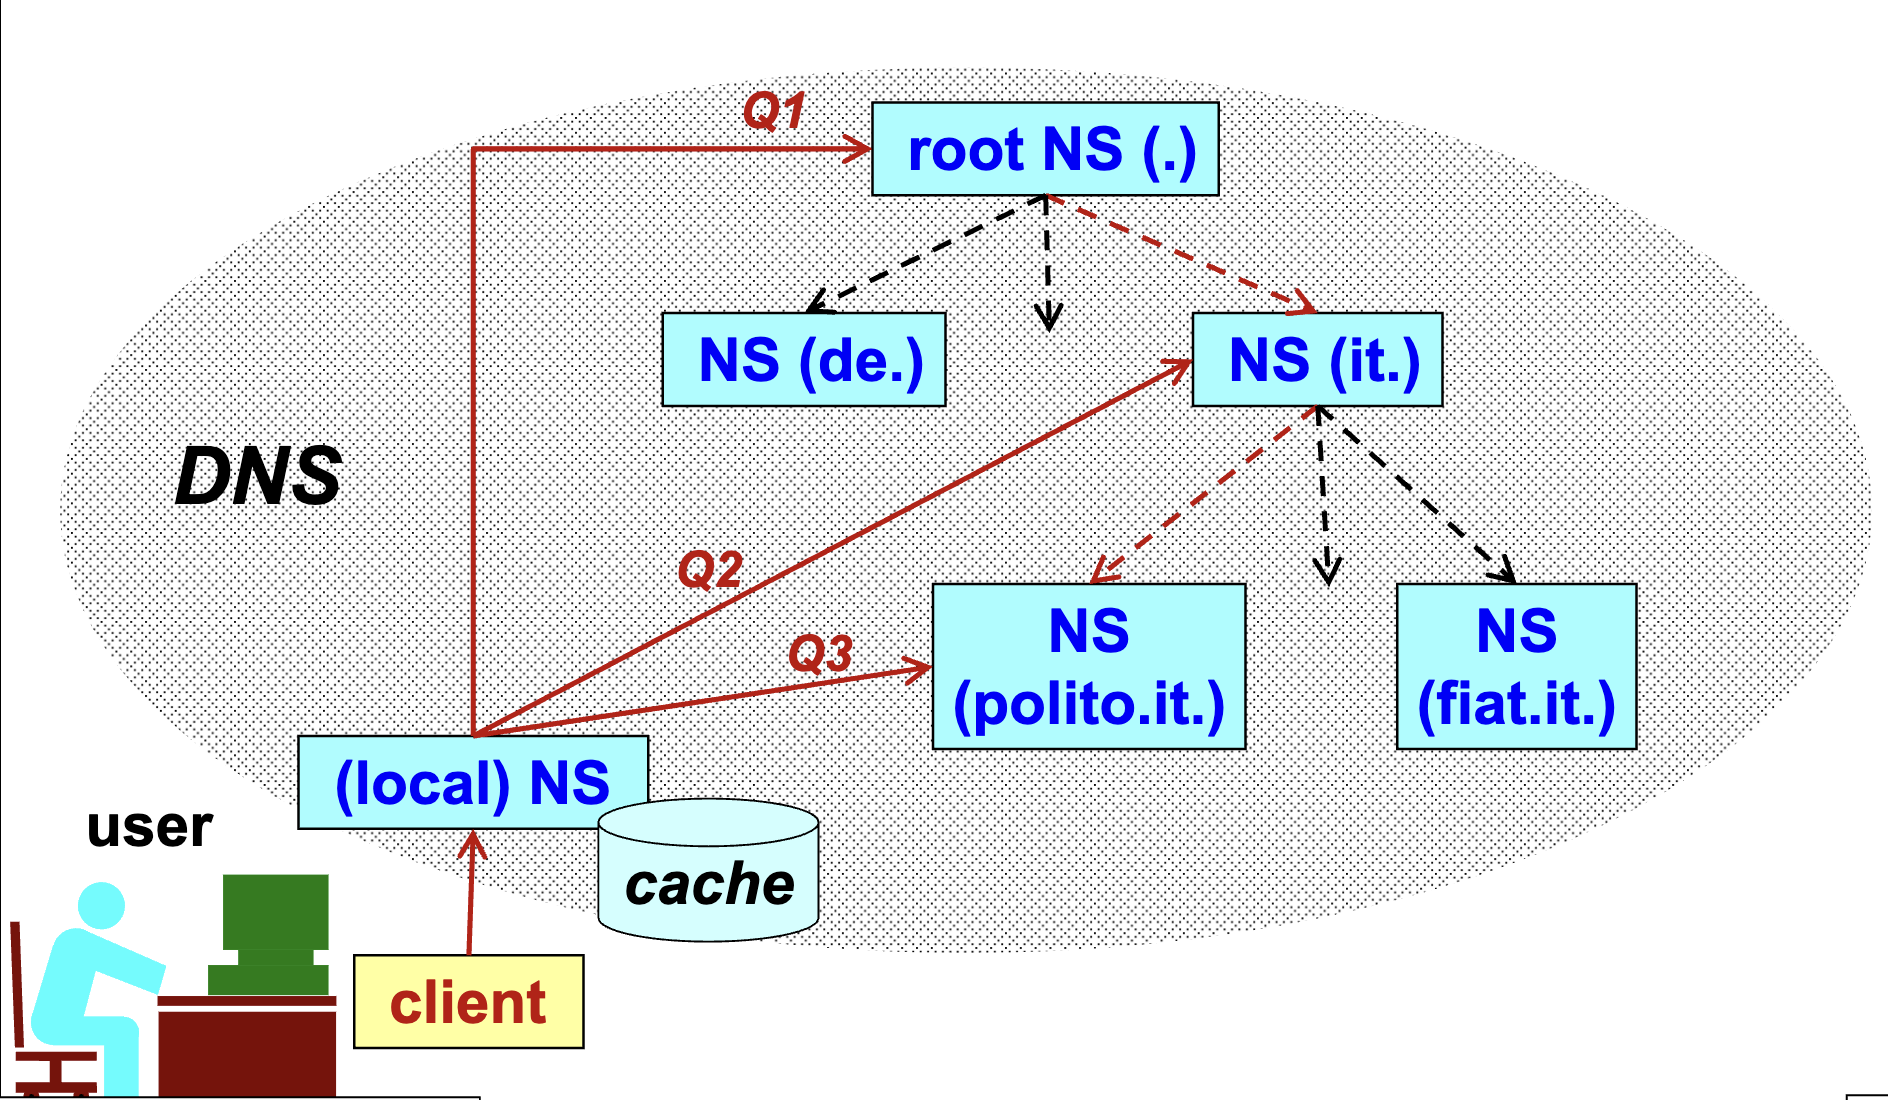
\includegraphics[width=0.6\linewidth]{Images/NetSec/dns_architecture.png}
  \caption{DNS architecture for iterative query.}
\end{figure}

\clearpage

\subsection*{DNS Shadow Server}
A DNS shadow server is a type of DNS server used for security, monitoring or malicious purposes. It is designed to closely mimic an authoritative DNS server but operates in the background without directly interacting with client queries.

\hfill


\textbf{Main passages of attacks:}
\begin{itemize}
    \item Sniffing to intercept queries.
    \item Spoofing to generate fake answers (e.g., Denial of Service or traffic redirection to fake sites).
\end{itemize}

If the attack occurs between nameservers, it can lead to a Distributed Denial of Service (DDoS) attack.
\begin{figure}[H]
    \centering
  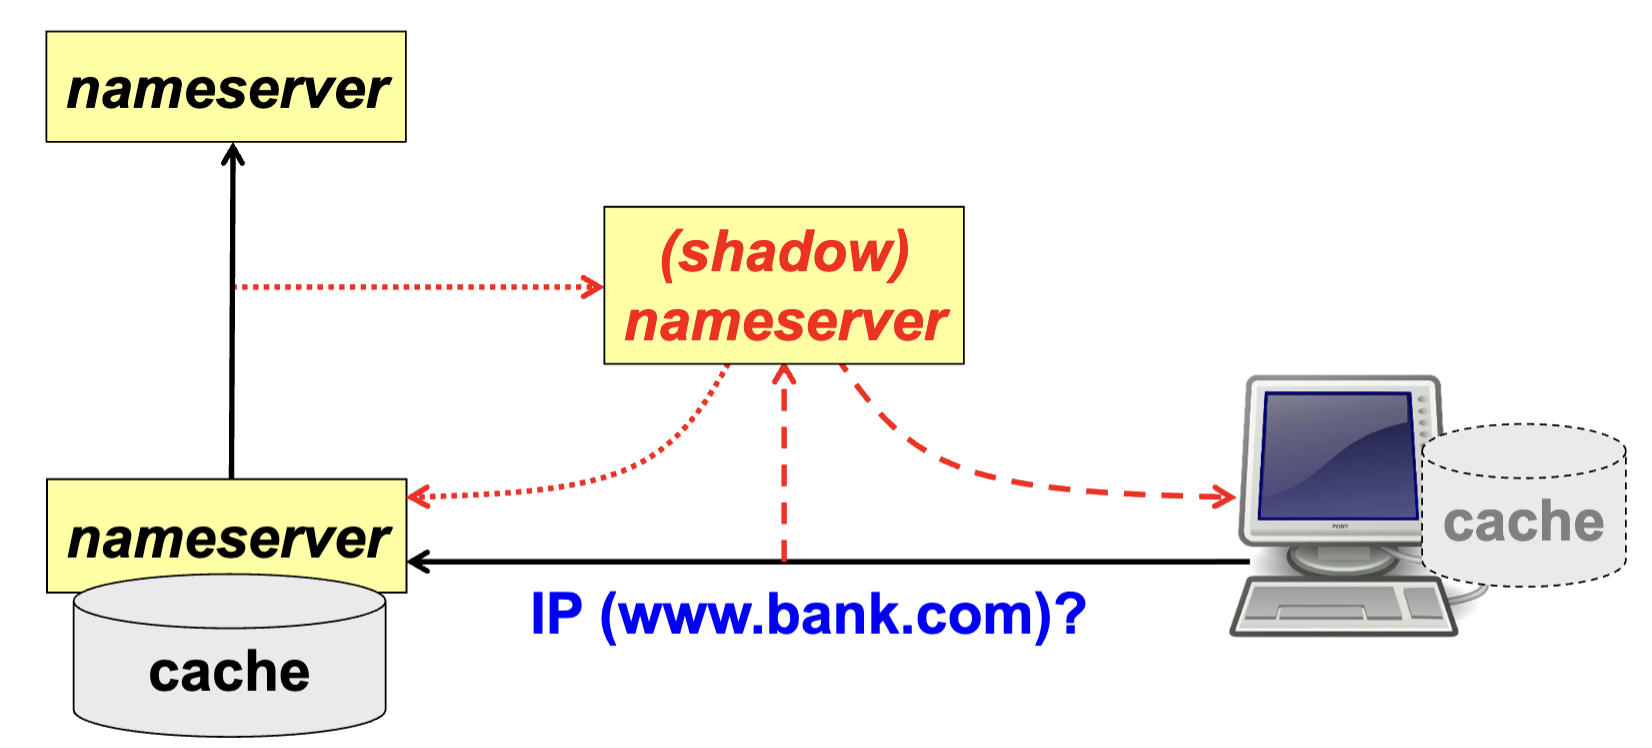
\includegraphics[width=0.6\linewidth]{Images/NetSec/dns_shadow_server.png}
  \caption{DNS shadow server usages.}
\end{figure}

\subsection{Name-address Translation}
This figure \ref{fig:name_address_trans} explains the vulnerabilities and security risks associated with the Name-Address Translation System, typically implemented in DNS (Domain Name System) architectures.

\begin{center}
    \textbf{The process:}
\end{center}
\begin{enumerate}
    \item App \#1 Initiates a Request: Wants to resolve a domain name (e.g., www.example.com) to an IP address. It sends the request to the Operating System (OS) through the Name Switch.
    \item Name Switch: 	The Name Switch in the OS determines how the domain name should be resolved. \textcolor{Red}{Unauthorized configurations because default options can be changed.} It checks the following in order:
    \begin{itemize}
        \item Local Data (e.g., /etc/hosts): If the name exists in local configuration files, it uses this data. \textcolor{Red}{Data corruption for the local data (e.g., file /etc/hosts)}
        \item If the name is not found locally, it forwards the query to the Resolver.
    \end{itemize}
    \item Resolver: The Resolver handles DNS queries on behalf of the OS. \textcolor{Red}{Unauthorized configurations, queries may be redirected to malicious servers.}
    \begin{itemize}
        \item It forwards the query to a (Recursive) Caching Server for further resolution. \textcolor{Red}{Server impersonation and no authentication, attackers may impersonate authoritative servers, providing fraudulent responses.}
    \end{itemize} 
    \item Recursive Caching Server: checks its Cache to see if it already has the requested domain name's IP address. \textcolor{Red}{Cache poisoning, attackers inject false data into the cache.}
    \begin{itemize}
        \item Cache Hit: If the result exists in the cache, it returns the IP address to the resolver.
        \item Cache Miss: If the result is not in the cache, it queries the authoritative DNS servers.
    \end{itemize}
    \item  Zone Master (Primary) and Zone Slave (Secondary):
    \begin{itemize}
        \item The Zone Master responds with the authoritative answer.
        \item The Zone Slave (Secondary) might also serve the query if it holds a copy of the zone file.
        \item Risks:
        \begin{itemize}
            \item \textcolor{Red}{Data Corruption}: Errors in the Zone File on the master or slave could propagate incorrect information.
            \item \textcolor{Red}{Unauthorized Updates}: Without proper authentication, attackers can modify the DNS records dynamically.
            \item \textcolor{Red}{Server Impersonation}: Attackers can masquerade as authoritative servers and inject false data.
        \end{itemize}
    \end{itemize}
    \item Response Propagation: Once the Recursive Caching Server obtains the correct IP address, it sends the result back to the Resolver. The Resolver delivers the resolved IP address to the Name Switch, which forwards it to App \#1.
\end{enumerate}

\begin{tcolorbox}[colback=blue!10!white, colframe=blue!50!white, title=Dynamic Updates]
    Dynamic updates simplify DNS management by allowing DNS records to be modified in real time, eliminating the need to manually edit zone files. This feature is particularly useful in dynamic network environments where devices frequently join or leave the network, such as with DHCP (Dynamic Host Configuration Protocol).
    How Dynamic Updates work:
    \begin{itemize}
        \item App (or Client) Requests an Update: When a device obtains an IP address from a DHCP server, it sends a request to register its hostname and IP address with the DNS server.
        \item Zone Master Handles the Update: The Zone Master (Primary) DNS server processes the request. The updated zone file may then be synchronized with any Zone Slaves (Secondary) to ensure consistency.
    \end{itemize}

    When \textcolor{Red}{no authentication mechanisms} are in place for dynamic updates, the system becomes vulnerable to \textcolor{Red}{unauthorized updates}.
\end{tcolorbox}

\begin{tcolorbox}[colback=red!10!white, colframe=red!70!black, coltitle=white, title=Beware]
    Query Privacy: Without encryption, the domain name query can be intercepted during transit.
\end{tcolorbox}
\begin{figure}[H]
  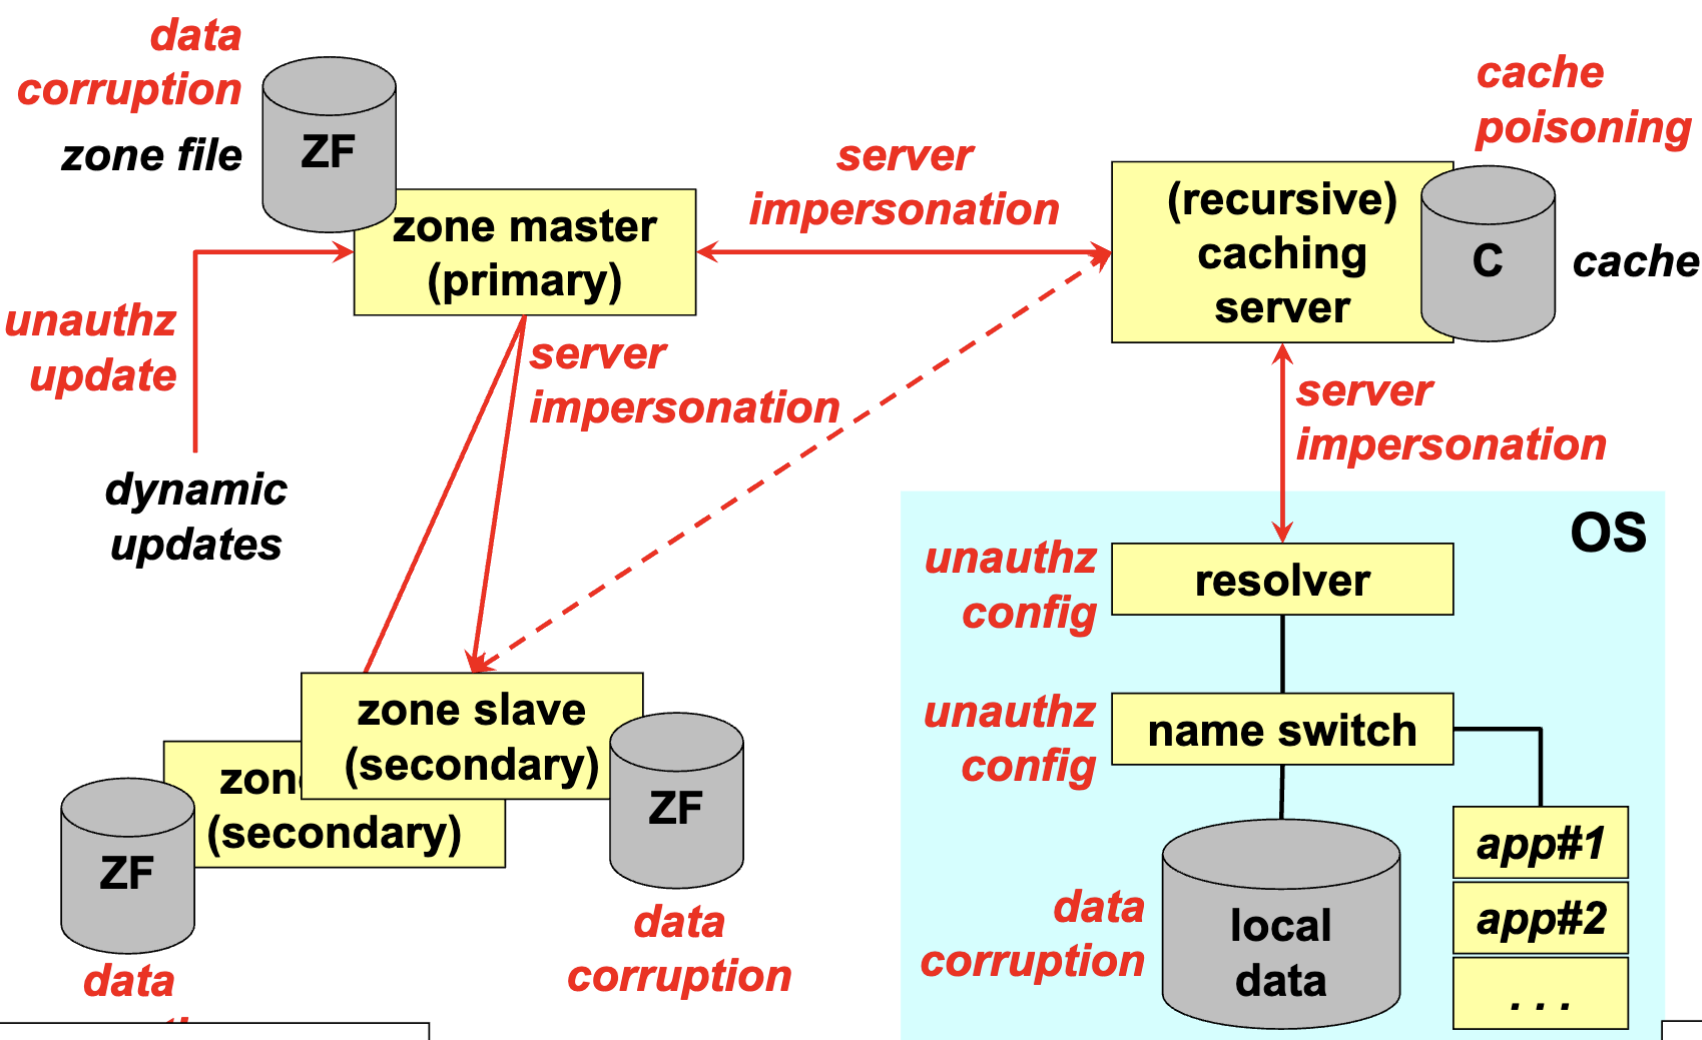
\includegraphics[width=\linewidth]{Images/NetSec/name_address_translation.png}
  \caption{Name-address translation process.}
  \label{fig:name_address_trans}
\end{figure}


\subsection{DoT and DoH}
\begin{center}
    (DNS-over-TLS \& DNS-over-HTTPS)
\end{center}

Apart from attacks against the nameservers, DNS has a \textbf{user privacy problem} for the queries:
\begin{itemize}
    \item Queries \textbf{can be read while in transit}.
    \item Queries \textbf{can be read and logged by the nameserver}.
\end{itemize}

\textbf{DNS-over-TLS (DoT)}:
\begin{itemize}
    \item Query and response are encapsulated in a secure \textbf{TLS tunnel}.
    \item However, it is still evident that it's a \textbf{DNS exchange}.
\end{itemize}

\textbf{DNS-over-HTTPS (DoH) (RFC-8484)}:
\begin{itemize}
    \item Query and response are part of a normal \textbf{HTTPS exchange}.
    \item Externally, it looks like visiting a secure web page.
\end{itemize}

\textbf{Well-known service providers of DoH/DoT}:
\begin{itemize}
    \item Cloudflare (\texttt{1.1.1.1}).
    \item Google (\texttt{8.8.8.8} and \texttt{8.8.4.4}).
\end{itemize}